\chapter{Cómo se ruteó la placa}\label{cap:ruteo}

% colores y estilos de las figuras generadas desde la placa (figuras/c09_*.tex)
\colorlet{fondo}{verdeplaca!6}\colorlet{padfill}{black!18}\colorlet{paddraw}{black!55}
\colorlet{cSW}{red!80!black}\colorlet{c24}{orange!90!black}\colorlet{cOut}{green!50!black}
\colorlet{cGND}{black!70}\colorlet{cSig}{blue!70!black}\colorlet{cIn}{violet}\colorlet{cB}{cyan!60!black}
\tikzset{etiq/.style={font=\sffamily\tiny\bfseries,text=black,fill=white,fill opacity=0.7,text opacity=1,inner sep=0.6pt}}

Con el placement fijo (capítulo~\ref{cap:placement}) y la placa ya en 4 capas (capítulo~\ref{cap:capas}), faltaba
lo más largo: dibujar las pistas. Aquí vas a ver las reglas que siguió cada pista, por qué existe cada regla, cómo se
dibujó la placa (no con un autorouter) y qué se decidió en cada uno de los diez bloques del ruteo.

\textbf{En este capítulo vas a ver:}
\begin{itemize}
  \item el método: pistas escritas como listas de puntos, por bloques, con verificación después de cada bloque;
  \item las reglas de trazado, una por una, con su porqué y cómo se comprueba;
  \item anchos de pista, separaciones, zonas de cobre y vías de cosido;
  \item el recorrido bloque por bloque, desde los buck hasta los teardrops y la serigrafía;
  \item en qué orden hay que correr los pasos finales y por qué ese orden importa.
\end{itemize}

% =====================================================================================================
\section{El método: polilíneas por bloques}\label{sec:c09-metodo}

\subsection{Por qué no un autorouter}

Un autorouter (como Freerouting) encuentra caminos, pero no entiende el circuito: no sabe que el lazo de entrada de un
buck tiene que ser diminuto, que un condensador de desacoplo tiene que ir pegado al pin, que el nodo \net{SUM} no
puede tener nada debajo, ni que una pista debe entrar al pad por el centro. Además deja quiebres, vías y desvíos que
luego hay que limpiar a mano. Por eso Freerouting solo se usó como \emph{oráculo} en copias de la placa, para
preguntar si existía solución con una regla (capítulo~\ref{cap:capas}). El ruteo real se hizo a mano.

\subsection{``A mano'', pero escrito como datos}

``A mano'' no quiere decir con el mouse en KiCad. Cada pista se escribió como una lista de puntos de paso (coordenadas
de KiCad en mm) en un archivo de Python por bloque. Los archivos están en la carpeta
\archivo{tools/ruteo/bloques/}. Por ejemplo, el comienzo del bloque 2 (entrada de \SI{24}{\volt}) se ve así:

\begin{small}
\begin{verbatim}
PISTAS = [
    # 24V_IN: J5.1 -> D1.2 (ánodo), recto
    ('Net-(D1-A)', 1.0, 'F.Cu', [(104.5, 103.6), (111.25, 103.6)]),
    # 24V_PROT: D1.1 (cátodo) -> D2.1
    ('24V_PROT', 1.0, 'F.Cu', [(111.25, 107.6), (111.25, 108.95),
                              (111.75, 109.45), (111.75, 110.95)]),
    ...
\end{verbatim}
\end{small}

Cada entrada es (red, ancho en mm, capa, puntos). Hay listas iguales para las vías (\texttt{VIAS}) y las zonas
(\texttt{ZONAS}). El script \archivo{tools/ruteo/polilineas.py} lee el bloque y lo escribe en la placa con la API de
KiCad (\texttt{pcbnew}). Antes de escribir nada \textbf{valida el bloque}: cada segmento tiene que ser múltiplo de
\ang{45}, medir al menos \SI{0.1}{\milli\meter} y girar \ang{0} o \ang{45} respecto del anterior. Si el bloque no es
válido, no toca la placa.

\begin{idea}[por qué escribir las pistas como datos]
\begin{itemize}
  \item \textbf{Se puede rehacer un bloque sin tocar el resto.} Cada bloque se guarda en un grupo de KiCad
  (\texttt{ruteo:<bloque>}). Al volver a aplicarlo, el script borra lo que tenía ese grupo y lo vuelve a escribir.
  \item \textbf{Cada coordenada tiene un comentario} que dice por qué la pista pasa por ahí (``entre los pads de
  \net{R22} y \net{R24}, \SI{0.325}{\milli\meter} a cada lado'').
  \item \textbf{Es revisable y repetible}: el ruteo queda en git como texto, y cualquier cambio se ve en un diff.
\end{itemize}
\end{idea}

\subsection{Verificar después de cada bloque}

Después de cada bloque se corrió \archivo{tools/ruteo/verificar_bloque.py}, que hace siempre lo mismo:
\begin{enumerate}
  \item DRC de KiCad con paridad esquemático--placa, todas las severidades, rellenando las zonas y guardando el relleno;
  \item ERC del esquemático;
  \item \archivo{revisar_pistas.py}, el revisor propio con los chequeos A--M (lo que el DRC no ve);
  \item imágenes de cada capa para mirar a ojo.
\end{enumerate}
Solo con todo en cero se hacía commit y se pasaba al bloque siguiente. Después del bloque 1 hubo una parada
obligatoria para que el dueño revisara en KiCad. El detalle de estas herramientas está en el capítulo~\ref{cap:verif}.

% =====================================================================================================
\section{Las reglas de trazado, una por una}\label{sec:c09-reglas}

\subsection{Solo ángulos de 45°}

\textbf{Qué:} cada segmento de pista es horizontal, vertical o diagonal a \ang{45}, y dos segmentos seguidos forman un
ángulo interior de \ang{135} o más. Nada de esquinas de \ang{90} ni agudas.

\textbf{Por qué:} a las frecuencias de esta placa una esquina de \ang{90} no cambia el comportamiento eléctrico de forma
apreciable, así que el motivo no es ``la esquina radia''. Los motivos reales son de fabricación y de orden: un ángulo
agudo deja una cuña estrecha de cobre o de separación que es difícil de grabar bien; las diagonales acortan los
recorridos frente a dos tramos a \ang{90}; y una regla uniforme hace la placa fácil de revisar. Además era una regla
pedida por el dueño.

\textbf{Cómo se comprueba:} con la regla propia \texttt{solo\_45} del archivo \archivo{pcb.kicad_dru}
(\texttt{track\_angle} mínimo de \ang{135}, error en el DRC), con la validación de \archivo{polilineas.py} y con los
chequeos A y B de \archivo{revisar_pistas.py}.

\begin{figure}[htbp]
\centering
\begin{tikzpicture}[scale=0.9]
  \begin{scope}
    \draw[line width=3pt,cobre] (0,0) -- (1.5,0) -- (2.5,1) -- (2.5,2);
    \node[font=\small,green!40!black] at (1.3,-0.5) {bien: \ang{135}};
  \end{scope}
  \begin{scope}[xshift=4cm]
    \draw[line width=3pt,cobre] (0,0) -- (2,0) -- (2,2);
    \node[font=\small,rojoojo] at (1.2,-0.5) {mal: \ang{90}};
  \end{scope}
  \begin{scope}[xshift=8cm]
    \draw[line width=3pt,cobre] (0,0) -- (2,0) -- (0.8,1.2);
    \node[font=\small,rojoojo] at (1.1,-0.5) {mal: \ang{45} (agudo)};
  \end{scope}
\end{tikzpicture}
\caption{Esquinas permitidas y prohibidas. La regla mide el ángulo \emph{interior} entre los dos segmentos.}
\label{fig:c09-angulos}
\end{figure}

\subsection{Entrar al pad por el centro y por su eje}

\textbf{Qué:} la pista termina en el centro del pad y llega paralela a uno de sus ejes. Si tiene que girar, el quiebre
queda \emph{fuera} del pad.

\textbf{Por qué:} el pad de un componente pequeño (un 0402 o un 0603) es casi del tamaño de la pista. Si la pista
entra en diagonal o por una esquina, el cobre ``visible'' del pad cambia de forma: la soldadura moja distinto a cada
lado y en las piezas chicas eso favorece que el componente se levante de un lado (efecto lápida o
\emph{tombstoning}). Entrar por el eje y por el centro hace que los dos pads de una pieza se vean iguales para la
soldadura. Además, una pista que sale de un pin fino con el ancho del pad no deja esquinas de cobre fuera del pad.

\textbf{Cómo se comprueba:} chequeo C de \archivo{revisar_pistas.py}. Hubo una sola excepción aceptada, el enlace del
nodo \net{SUM} entre el condensador de realimentación y la resistencia de entrada (bloque 5).

\begin{figure}[htbp]
\centering
\begin{tikzpicture}[scale=0.9]
  \tikzset{pad/.style={fill=black!18,draw=black!55,rounded corners=1pt}}
  \begin{scope}
    \draw[pad] (0,0) rectangle (1,1.2);
    \draw[line width=4pt,cobre] (0.5,0.6) -- (2.5,0.6) -- (3.3,1.4);
    \fill (0.5,0.6) circle (0.05);
    \node[font=\small,green!40!black,align=center] at (1.6,-0.5) {bien: llega por el eje,\\quiebre fuera del pad};
  \end{scope}
  \begin{scope}[xshift=5cm]
    \draw[pad] (0,0) rectangle (1,1.2);
    \draw[line width=4pt,cobre] (0.5,0.6) -- (1.8,1.9);
    \node[font=\small,rojoojo,align=center] at (1.1,-0.5) {mal: entra\\en diagonal};
  \end{scope}
  \begin{scope}[xshift=9cm]
    \draw[pad] (0,0) rectangle (1,1.2);
    \draw[line width=4pt,cobre] (0.9,0.2) -- (2.5,0.2);
    \node[font=\small,rojoojo,align=center] at (1.3,-0.5) {mal: termina\\fuera del centro};
  \end{scope}
\end{tikzpicture}
\caption{Entrada de una pista a un pad. Solo la primera cumple el chequeo C.}
\label{fig:c09-entrada}
\end{figure}

\subsection{Sin \emph{stubs}}

\textbf{Qué:} ninguna pista termina en el aire ni sigue de largo después de su último punto de conexión. Tampoco hay
segmentos duplicados o superpuestos, ni vías que no conecten al menos dos capas.

\textbf{Por qué:} un tramo que no lleva a ningún lado (\emph{stub}) no conduce corriente útil, pero sí tiene capacidad y
se comporta como una pequeña antena que capta ruido. En señales rápidas, un stub refleja la señal. Y casi siempre es
un error: un pedazo de pista que quedó de una edición anterior.

\textbf{Cómo se comprueba:} chequeos E y F de \archivo{revisar_pistas.py} y las reglas \texttt{track\_dangling} y
\texttt{via\_dangling} del DRC, configuradas como error.

\subsection{Ramificar solo en pads o en zonas}

\textbf{Qué:} si una red tiene que repartirse a varias piezas, la división se hace en el pad de una pieza (o en una
zona de cobre), nunca en medio de una pista.

\textbf{Por qué:} una ``T'' en medio de una pista crea un ángulo de \ang{90} entre ramas, y con tres ramas en un punto
no pueden quedar todas a \ang{135} o más entre sí. El DRC de KiCad mide eso con \texttt{track\_angle} y lo marca. Se
descubrió al probar el bus de \SI{24}{\volt} en una copia de la placa: una unión en T sobre pista desnuda la marcó el DRC.

Hubo un caso más sutil en el bloque 8: la regla \texttt{track\_angle} también mira las uniones \emph{en vías}. Una vía
con tres pistas en la misma capa tiene el mismo problema que la T. Por eso el pad \net{R9.2} tiene \textbf{dos vías}
unidas por \capa{F.Cu}, y de cada una sale una sola rama.

\begin{figure}[htbp]
\centering
\begin{tikzpicture}[scale=0.9]
  \tikzset{pad/.style={fill=black!18,draw=black!55,rounded corners=1pt}}
  \begin{scope}
    \draw[line width=3pt,cobre] (0,0) -- (3,0);
    \draw[line width=3pt,cobre] (1.5,0) -- (1.5,1.4);
    \node[font=\small,rojoojo] at (1.5,-0.5) {mal: T en pista};
  \end{scope}
  \begin{scope}[xshift=5cm]
    \draw[pad] (1.1,-0.4) rectangle (1.9,0.4);
    \draw[line width=3pt,cobre] (0,0) -- (1.5,0) -- (3,0);
    \draw[line width=3pt,cobre] (1.5,0) -- (1.5,1.4);
    \node[font=\small,green!40!black] at (1.5,-0.8) {bien: la unión es el pad};
  \end{scope}
\end{tikzpicture}
\caption{Una ramificación en pista libre deja un ángulo de \ang{90}. Si la unión cae en el centro de un pad, la
``esquina'' queda dentro del cobre del pad y no hay ángulo de pista.}
\label{fig:c09-t}
\end{figure}

\subsection{Teardrops}

\textbf{Qué:} un \emph{teardrop} (lágrima) es un relleno triangular de cobre en la unión entre una pista y un pad o una
vía, que ensancha la pista justo antes de llegar.

\textbf{Por qué:} la unión pista--pad es el punto mecánicamente más débil. Si el taladro sale un poco corrido (todos los
fabricantes tienen tolerancia de registro), el anillo de cobre alrededor del agujero puede quedar muy angosto justo
donde llega la pista, y la pista se puede cortar. El teardrop agrega cobre ahí y también reparte el esfuerzo térmico y
mecánico.

\textbf{Cómo se hizo:} \archivo{tools/ruteo/teardrops.py} activa los teardrops en todos los pads con red y en todas las
vías, con los parámetros por defecto de KiCad 10. No hace falta abrir KiCad: el DRC por línea de comandos con
\texttt{-{}-refill-zones -{}-save-board} genera las zonas de teardrop. Resultado: \textbf{440 teardrops} \medido.

\begin{figure}[htbp]
\centering
\begin{tikzpicture}[scale=1]
  \begin{scope}
    \fill[black!18] (0,0) circle (0.6); \fill[white] (0,0) circle (0.25);
    \draw[line width=4pt,cobre] (0.5,0) -- (2.6,0);
    \node[font=\small] at (1.2,-0.9) {sin teardrop};
  \end{scope}
  \begin{scope}[xshift=4.5cm]
    \fill[cobre!70] (0.35,0.45) .. controls (0.9,0.3) and (1.3,0.08) .. (1.7,0.07) -- (1.7,-0.07) .. controls (1.3,-0.08) and (0.9,-0.3) .. (0.35,-0.45) -- cycle;
    \fill[black!18] (0,0) circle (0.6); \fill[white] (0,0) circle (0.25);
    \draw[line width=4pt,cobre] (0.5,0) -- (2.6,0);
    \node[font=\small] at (1.2,-0.9) {con teardrop};
  \end{scope}
\end{tikzpicture}
\caption{Unión pista--vía sin y con teardrop. El relleno refuerza la zona donde un taladro corrido dejaría el anillo
más angosto.}
\label{fig:c09-teardrop}
\end{figure}

\subsection{Desacoplo pegado al pin, con su vía GND al lado}

\textbf{Qué:} cada condensador de desacoplo queda a \SI{1.0}{\milli\meter} o menos (borde a borde) del pin que desacopla
(chequeo L), y el pad GND del condensador tiene su vía al plano a \SI{1.0}{\milli\meter} o menos (chequeo K). Lo mismo
para cada pin GND SMD de los integrados.

\textbf{Por qué:} un integrado pide corriente en pulsos muy cortos (cada vez que conmuta algo adentro). Esa corriente
no puede venir desde el buck, que está lejos y detrás de pistas con inductancia: la entrega el condensador de
desacoplo, que es una ``reserva'' local. Para que funcione, el lazo condensador $\to$ pin de alimentación $\to$ pin de
GND $\to$ plano $\to$ condensador tiene que ser chico (sección~\ref{sec:c08-area}). Cada milímetro de más es
inductancia en serie con el condensador, y por encima de cierta frecuencia el condensador deja de servir. La nota de
ADI MT-101 lo dice así: \SIrange{0.01}{0.1}{\micro\farad} lo más cerca posible del pin, unido al plano con vía o pista
corta \doc{MT-101}.

\begin{figure}[htbp]
\centering
\begin{tikzpicture}[scale=0.85]
  \tikzset{pad/.style={fill=black!18,draw=black!55,rounded corners=1pt}}
  \begin{scope}
    \draw[pad] (0,0) rectangle (2,2.4); \node[font=\small] at (1,1.2) {IC};
    \draw[pad] (2,1.75) rectangle (2.5,2.05);
    \draw[pad] (2.75,1.6) rectangle (3.3,2.2); \draw[pad] (3.65,1.6) rectangle (4.2,2.2);
    \draw[line width=2.5pt,cobre] (2.5,1.9) -- (2.95,1.9);
    \filldraw[fill=cGND,draw=black] (4.6,1.9) circle (0.17); \fill[white] (4.6,1.9) circle (0.08);
    \draw[line width=2.5pt,black!70] (3.95,1.9) -- (4.45,1.9);
    \node[font=\small,green!40!black,align=center] at (2.3,-0.6) {bien: C junto al pin,\\vía GND al lado};
  \end{scope}
  \begin{scope}[xshift=6.6cm]
    \draw[pad] (0,0) rectangle (2,2.4); \node[font=\small] at (1,1.2) {IC};
    \draw[pad] (2,1.75) rectangle (2.5,2.05);
    \draw[pad] (4.4,0.6) rectangle (4.95,1.2); \draw[pad] (5.3,0.6) rectangle (5.85,1.2);
    \draw[line width=2.5pt,cobre] (2.5,1.9) -- (3.6,1.9) -- (4.3,1.2) -- (4.65,0.9);
    \filldraw[fill=cGND,draw=black] (5.6,-0.4) circle (0.17); \fill[white] (5.6,-0.4) circle (0.08);
    \draw[line width=2.5pt,black!70] (5.6,0.9) -- (5.6,-0.23);
    \node[font=\small,rojoojo,align=center] at (2.6,-1.1) {mal: C lejos y vía lejos\\(lazo grande)};
  \end{scope}
\end{tikzpicture}
\caption{Desacoplo. A la izquierda el lazo pin--condensador--vía--plano es mínimo; a la derecha cada milímetro extra suma
inductancia y el condensador pierde efecto a alta frecuencia.}
\label{fig:c09-desacoplo}
\end{figure}

\begin{ojo}[cuando no se pudo cumplir]
Algunos condensadores quedaron a más de \SI{1.0}{\milli\meter} y se aceptaron como excepciones: \net{C36}/\net{C46}
(VCC de los buck, \SI{3.0}{\milli\meter}), los condensadores de entrada de los LT3092 (\net{C2}, \net{C3}, \net{C49},
\net{C50}), los del PCM1808 (\net{C11}, \net{C12}, \net{C15}, \net{C16}, \net{C18}), y los del MCP4725, que se juzgan
con el límite de su datasheet (\SI{4}{\milli\meter} \doc{DS22039D §8.3}). La lista completa y el motivo de cada una
está en el capítulo~\ref{cap:banco}.
\end{ojo}

\subsection{Vías taponadas a \SI{0.35}{\milli\meter} o más de los pads}

\textbf{Qué:} ninguna vía queda a menos de \SI{0.35}{\milli\meter} de un pad (de cualquier red).

\textbf{Por qué:} en placas de 4 capas JLCPCB tapona las vías por defecto (\emph{plugged}): rellena el agujero con tinta
de máscara. Su artículo de recubrimiento de vías dice que ``vias with a distance less than 0.35mm from the pad cannot
be plugged with ink'' \doc{JLCPCB}. Una vía mal tapada junto a un pad puede chupar soldadura del pad durante el
reflujo y dejar la unión pobre.

\textbf{Cómo se hizo:} una regla propia en \archivo{pcb.kicad_dru}:
\begin{small}
\begin{verbatim}
(rule "via_tapada_lejos_de_pad"
  (condition "A.Type == 'Via' && B.Type == 'Pad'")
  (constraint physical_clearance (min 0.35mm)))
\end{verbatim}
\end{small}
Cuando se agregó (después del bloque 4) ya había vías puestas; 43 de ellas violaban la regla. Se corrieron con ayuda
de \archivo{tools/ruteo/sugerir_vias.py}, que prueba posiciones sobre los cuatro ejes del pad, entre
\SI{0.35}{\milli\meter} y \SI{1.0}{\milli\meter} del borde (para seguir cumpliendo el chequeo K), y elige la más
cercana que respeta todas las separaciones. En los buck, las vías de los condensadores de entrada y salida pasaron
bajo el cuerpo del condensador. \net{C19} se quedó sin vía propia porque no había ningún lugar legal: su pad GND lo une
el relleno de \capa{F.Cu}.

\subsection{Anchos de pista}

Cada red pertenece a una \emph{clase} con su ancho y su separación mínimos (\archivo{pcb.kicad_pro}):

\begin{center}
\begin{tabular}{@{}lccl@{}}
\toprule
\textbf{Clase} & \textbf{Ancho} & \textbf{Separación} & \textbf{Ejemplos} \\
\midrule
Default & \SI{0.2}{\milli\meter} & \SI{0.2}{\milli\meter} & I2C, straps \\
Analógica & \SI{0.2}{\milli\meter} & \SI{0.3}{\milli\meter} & \net{IEPE}, \net{SUM}, \net{REST_OUT}, \net{DC_MON} \\
Reloj & \SI{0.2}{\milli\meter} & \SI{0.3}{\milli\meter} & \net{SAI_SCK}, \net{SAI_FS}, MCLK del ADC \\
Potencia & \SI{0.25}{\milli\meter} & \SI{0.2}{\milli\meter} & \net{24V_PROT}, \net{3V3}, \net{5V_A}, GND \\
Conmutado & \SI{0.25}{\milli\meter} & \SI{0.2}{\milli\meter} & \net{SW_3}, \net{SW_5} \\
\bottomrule
\end{tabular}
\end{center}

Todas las clases usan vías de \SI{0.6}{\milli\meter} de diámetro con taladro de \SI{0.3}{\milli\meter}. La regla
propia \texttt{ancho\_minimo\_potencia} hace que el DRC marque como error cualquier pista de Potencia o Conmutado más
angosta que \SI{0.25}{\milli\meter}.

\begin{idea}[el ancho lo fija la fabricación, no la corriente]
En el plan inicial las clases de potencia tenían \SI{0.5}{\milli\meter}, que resultó ser el valor por defecto de
KiCad y no un cálculo. Con IPC-2221 (\SI{10}{\celsius} de calentamiento) la pista más exigida, el nodo \net{SW} con
\SI{275}{\milli\ampere} de pico, necesitaría solo \SI{0.051}{\milli\meter}; el bus de \SI{24}{\volt} con
\SI{50}{\milli\ampere}, \SI{0.005}{\milli\meter} \doc{CALCULOS.md §3} \copia[fórmula IPC]. Por eso las pistas de
potencia van de \SIrange{0.25}{1.0}{\milli\meter}: el mínimo lo pone la regla de clase, y donde hay lugar se
ensanchan (el camino del TVS va a \SI{1.0}{\milli\meter}, la pista \net{SW} a la bobina a \SI{0.6}{\milli\meter}).
Las salidas de los pines de los integrados finos van con el ancho del pad (\SI{0.25}{\milli\meter}) y se ensanchan
fuera de él. Los números completos están en el capítulo~\ref{cap:calculos}.
\end{idea}

\subsection{Separaciones especiales}

Además de la separación de cada clase, \archivo{pcb.kicad_dru} tiene dos reglas para alejar lo ruidoso de lo sensible:
\begin{itemize}
  \item \texttt{sw\_lejos\_de\_analogica}: \SI{1}{\milli\meter} entre una red Conmutada (los nodos \net{SW}, que saltan
  \SI{24}{\volt} en nanosegundos) y cualquier red Analógica.
  \item \texttt{reloj\_lejos\_de\_analogica}: \SI{0.5}{\milli\meter} entre una red de Reloj y una Analógica.
\end{itemize}
La razón es el acople capacitivo: la capacidad entre dos pistas baja cuando se separan, y con ella el ruido que pasa
(sección~\ref{sec:c08-altaz}). El chequeo J de \archivo{revisar_pistas.py} añade una regla más: una pista analógica no
puede ir en paralelo a una digital o de reloj a menos de \SI{1}{\milli\meter} por más de \SI{2}{\milli\meter}, en
ninguna capa.

\subsection{Zonas de cobre y sus prioridades}

Una \emph{zona} es un polígono de cobre que KiCad rellena automáticamente, apartándose de lo que no es de su red.
Cuando dos zonas se superponen, gana la de mayor \emph{prioridad}. Las zonas de la placa \medido:

\begin{center}
\begin{tabular}{@{}llcl@{}}
\toprule
\textbf{Zona} & \textbf{Capa} & \textbf{Prioridad} & \textbf{Para qué} \\
\midrule
\texttt{SW\_3\_PIN3}, \texttt{SW\_5\_PIN3} & \capa{F.Cu} & 3 & unir el pin 3 (NC) con el pin 12 (SW) del buck \\
\texttt{VOUT\_3V3}, \texttt{VOUT\_5V} & \capa{F.Cu} & 2 & salida de la bobina y condensadores de salida \\
\texttt{BUS\_24V} & \capa{F.Cu} & 1 & bus de \SI{24}{\volt} a los condensadores de entrada \\
\texttt{GND\_FCU} & \capa{F.Cu} & 0 & relleno GND en todo lo libre \\
\texttt{GND\_IN1} & \capa{In1.Cu} & 0 & plano GND entero \\
\texttt{GND\_BCU} & \capa{B.Cu} & 0 & GND alrededor de las pistas lentas \\
\bottomrule
\end{tabular}
\end{center}

El relleno GND de \capa{F.Cu} tiene la prioridad más baja para que \emph{ceda} ante las zonas de potencia: rellena todo
lo que queda libre, pero nunca se mete en una zona de \SI{24}{\volt} o de \net{SW}.

\textbf{Conexión de los pads a la zona.} Hay dos formas de unir un pad a una zona de su red:
\begin{itemize}
  \item \textbf{sólida}: el pad queda rodeado de cobre por completo. Es la mejor conexión eléctrica (baja resistencia e
  inductancia). Se usó en todos los pads SMD, en particular en los pads GND de los condensadores de entrada y salida y
  en los pines PGND de los buck, que llevan la corriente conmutada;
  \item \textbf{alivio térmico}: el pad se une a la zona por unos pocos ``rayos'' finos. Se usa \textbf{solo en los
  pads con agujero (THT)}, que se sueldan a mano: con una unión sólida, el plano se lleva el calor del cautín y la
  soldadura no moja bien. Las piezas SMD las suelda JLCPCB en un horno de reflujo, donde toda la placa se calienta
  pareja, así que no lo necesitan.
\end{itemize}
El script \archivo{tools/ruteo/conexion_solida.py} comprueba que en cada buck los 10 pads GND de potencia (condensadores
de entrada, de alta frecuencia, de salida y los pines PGND) estén enteros dentro de la misma isla del relleno, sin
rayos.

\textbf{Sin islas.} Un pedazo de cobre que no está unido a nada (una isla) es una antena flotante. Las zonas eliminan
las islas y el DRC tiene \texttt{isolated\_copper} como error.

\subsection{Vías de cosido}

Las \emph{vías de cosido} (\emph{stitching vias}) son vías GND que no conectan ninguna pieza: unen el relleno GND de
\capa{F.Cu} con los planos de \capa{In1.Cu} y \capa{B.Cu} en muchos puntos. Así el relleno de \capa{F.Cu} no queda como
una lámina conectada solo en un par de lugares, y la corriente de retorno tiene siempre una vía cerca cuando necesita
cambiar de capa. \archivo{tools/ruteo/cosido.py} las propone así:
\begin{itemize}
  \item un anillo a \SI{1.2}{\milli\meter} del borde, una vía cada \SI{5}{\milli\meter};
  \item una grilla de \SI{2.5}{\milli\meter} en la zona del AFE y del ADC, y de \SI{5}{\milli\meter} en el resto;
  \item cada candidata se descarta si no cumple \emph{en las cuatro capas} (la vía las atraviesa todas):
  \SI{0.35}{\milli\meter} de todo pad, separación de clase a pistas y vías de otras redes, fuera de las zonas de
  potencia, \SI{0.8}{\milli\meter} del borde y \SI{0.15}{\milli\meter} de toda la serigrafía.
\end{itemize}
Quedaron \textbf{235 vías de cosido}. Contando todas, la placa tiene \textbf{329 vías}, de las cuales 299 son GND
\medido.

% =====================================================================================================
\section{Bloque por bloque}\label{sec:c09-bloques}

El ruteo se hizo en diez bloques, en un orden pensado para que lo más crítico tuviera el mejor lugar: primero las
fuentes conmutadas (que más ruido generan), luego la entrada, las fuentes IEPE, el ADC, el AFE, las analógicas largas,
lo digital, la alimentación y al final la tierra, los teardrops y la serigrafía.

\subsection{Bloque 1: los buck \net{U6} (3,3 V) y \net{U7} (5 V)}

\begin{idea}[el lazo caliente de un buck]
En un buck la corriente de la \emph{bobina} es continua (sube y baja en triángulo), pero la corriente de \emph{entrada}
es pulsada: cuando conduce el interruptor de arriba, toda la corriente de la bobina sale del condensador de entrada;
cuando conduce el de abajo, cae a cero de golpe. Ese lazo, condensador de entrada $\to$ \net{VIN} $\to$ interruptores
$\to$ \net{PGND} $\to$ condensador, tiene el $di/dt$ más grande de toda la placa. Se llama \textbf{lazo caliente}, y es
lo primero que se dibuja y lo que tiene que ser más chico. El datasheet lo pide así: el lazo de entrada corto, ancho y de
área mínima, y un condensador de \SI{220}{\nano\farad} lo más cerca posible de \emph{cada} par \net{VIN}/\net{PGND}
(pines 2/1 y 10/11) \doc{SNVSB49D §12.1 p.34}.
\end{idea}

\begin{figure}[htbp]
\centering
\begin{circuitikz}[scale=0.95,transform shape]
  \draw (0,0) to[C,l=$C_\text{IN}$] (0,3) to[nos,l=$Q_1$] (4.4,3);
  \draw (0,0) -- (4.4,0);
  \draw (4.4,3) to[nos,l=$Q_2$,*-*] (4.4,0);
  \draw (4.4,3) to[L,l=$L$] (7.4,3) to[C,l=$C_\text{OUT}$] (7.4,0) -- (4.4,0);
  \draw (6.0,0) node[ground]{};
  \draw[line width=6pt,rojoojo,opacity=0.25,rounded corners] (0.25,0.25) rectangle (4.15,2.75);
  \node[rojoojo,font=\small,align=center] at (2.2,1.45) {lazo caliente\\(corriente pulsada)};
  \node[font=\small] at (-0.6,3.3) {\net{VIN}};
  \node[font=\small] at (4.4,3.4) {\net{SW}};
  \node[font=\small] at (2.2,-0.35) {\net{PGND}};
\end{circuitikz}
\caption{Esquema simplificado de un buck. El lazo de entrada (rojo) cambia de corriente de golpe en cada conmutación;
el lazo de salida, a través de la bobina, lleva una corriente triangular continua y es menos crítico.}
\label{fig:c09-lazo-buck}
\end{figure}

Lo que se hizo, siguiendo la figura~12-2 del datasheet \doc{SNVSB49D}:
\begin{itemize}
  \item \textbf{Todo el lazo de potencia en \capa{F.Cu}} (entrada, \net{SW}, bobina, salida), con zonas para la salida
  (\texttt{VOUT\_3V3}, \texttt{VOUT\_5V}). \net{U7} es exactamente el mismo dibujo que \net{U6}, desplazado
  \SI{21.6}{\milli\meter}.
  \item \textbf{Medidas del lazo caliente} con \archivo{tools/ruteo/medir.py} \medido: \net{PGND} (pin 1) a su condensador
  de \SI{220}{\nano\farad} \net{C29} por \SI{2.61}{\milli\meter} de pista, y el pin 11 a \net{C30} por
  \SI{2.21}{\milli\meter}. Los lazos \net{VIN}--CHF--\net{PGND} miden \SI{7.25}{\milli\meter} de perímetro y
  \SI{3.32}{\milli\meter\squared} de área de un lado, y \SI{6.97}{\milli\meter} y \SI{2.69}{\milli\meter\squared} del
  otro. Para que entraran, \net{C29}/\net{C39} subieron \SI{0.3}{\milli\meter} y \net{C35}/\net{C45} (CBOOT) pasaron a
  la izquierda del integrado.
  \item \textbf{Pin 3 unido a \net{SW} (pin 12)} como pide el datasheet \doc{SNVSB49D §12.1 ítem 3}, con una zona
  chica de \net{SW} (prioridad 3): con pistas no se podía entrar al centro del pin 12 sin un giro de \ang{90}.
  \item \textbf{BOOT}: sale por la izquierda del pin 4 y baja por fuera del cobre de \net{SW} hasta \net{C35}.
  \item \textbf{VCC}: \net{C36} quedó a \SI{3.0}{\milli\meter} del pin 5. Se aceptó con la pista de VCC a
  \SI{0.3}{\milli\meter}, la vía GND pegada a \net{C36.2} y un retorno corto por \capa{F.Cu} al pin de tierra analógica.
  \item \textbf{Realimentación (FB)}: \net{R29}/\net{R30} junto al pin 7; el sensado de la salida llega desde abajo,
  lejos de \net{SW}. El nodo FB entero mide \SI{5.49}{\milli\meter} de cobre \medido.
  \item \textbf{Puentes en \capa{B.Cu}}: tres puentes de unos \SI{2.2}{\milli\meter} debajo del bus de
  \SI{24}{\volt}: el tronco de \net{3V3} y los dos sensados de FB. Solo cruzan potencia con potencia.
  \item \textbf{13 vías GND por buck}, junto a cada pad GND.
\end{itemize}

\begin{figure}[htbp]
\centering
% generado por tikz_zona.py, ventana KiCad (119.0,100.5)-(145.0,121.5) mm, 0.55 cm/mm
\begin{tikzpicture}[line cap=round,line join=round]
\clip (0,0) rectangle (14.300,11.550);
\fill[fondo] (0,0) rectangle (14.300,11.550);
\fill[c24,opacity=0.35] (21.569,2.527) -- (21.576,2.525) -- (21.603,2.505) -- (21.603,2.505) -- (21.605,2.503) -- (21.615,2.471) -- (21.615,2.126) -- (21.612,2.109) -- (21.610,2.102) -- (21.590,2.075) -- (21.588,2.073) -- (21.556,2.062) -- (1.328,2.062) -- (1.311,2.065) -- (1.304,2.067) -- (1.277,2.087) -- (1.277,2.087) -- (1.275,2.089) -- (1.265,2.121) -- (1.265,2.467) -- (1.268,2.484) -- (1.270,2.491) -- (1.290,2.518) -- (1.290,2.518) -- (1.292,2.520) -- (1.324,2.530) -- (21.552,2.530) -- cycle;
\fill[cOut,opacity=0.35] (23.549,11.520) -- (23.556,11.518) -- (23.583,11.498) -- (23.583,11.498) -- (23.585,11.496) -- (23.595,11.464) -- (23.595,10.073) -- (23.592,10.056) -- (23.590,10.049) -- (23.570,10.022) -- (23.568,10.020) -- (23.536,10.010) -- (22.118,10.010) -- (22.118,10.010) -- (22.118,10.010) -- (22.102,10.013) -- (22.095,10.015) -- (22.088,10.020) -- (22.086,10.020) -- (22.086,10.021) -- (22.067,10.035) -- (22.067,10.035) -- (22.066,10.037) -- (22.055,10.069) -- (22.055,10.074) -- (22.055,10.074) -- (22.037,10.144) -- (22.037,10.144) -- (22.037,10.144) -- (22.001,10.205) -- (22.000,10.206) -- (22.000,10.206) -- (22.000,10.207) -- (22.000,10.207) -- (21.949,10.258) -- (21.949,10.258) -- (21.949,10.258) -- (21.949,10.258) -- (21.918,10.276) -- (21.906,10.289) -- (21.859,10.301) -- (21.859,10.301) -- (21.828,10.310) -- (21.816,10.313) -- (21.816,10.313) -- (21.744,10.313) -- (21.744,10.313) -- (21.722,10.307) -- (21.701,10.301) -- (21.701,10.301) -- (21.674,10.294) -- (21.674,10.294) -- (21.611,10.258) -- (21.560,10.207) -- (21.523,10.144) -- (21.523,10.144) -- (21.523,10.144) -- (21.505,10.074) -- (21.505,10.074) -- (21.505,10.073) -- (21.502,10.056) -- (21.500,10.049) -- (21.480,10.022) -- (21.478,10.020) -- (21.446,10.010) -- (20.138,10.010) -- (20.138,10.010) -- (20.138,10.010) -- (20.122,10.013) -- (20.115,10.015) -- (20.108,10.020) -- (20.106,10.020) -- (20.106,10.021) -- (20.087,10.035) -- (20.087,10.035) -- (20.086,10.037) -- (20.075,10.069) -- (20.075,10.074) -- (20.075,10.074) -- (20.057,10.144) -- (20.057,10.144) -- (20.057,10.144) -- (20.021,10.205) -- (20.020,10.206) -- (20.020,10.206) -- (20.020,10.207) -- (20.020,10.207) -- (19.969,10.258) -- (19.969,10.258) -- (19.969,10.258) -- (19.969,10.258) -- (19.938,10.276) -- (19.926,10.289) -- (19.879,10.301) -- (19.879,10.301) -- (19.848,10.310) -- (19.836,10.313) -- (19.836,10.313) -- (19.764,10.313) -- (19.764,10.313) -- (19.742,10.307) -- (19.721,10.301) -- (19.721,10.301) -- (19.694,10.294) -- (19.694,10.294) -- (19.631,10.258) -- (19.580,10.207) -- (19.543,10.144) -- (19.543,10.144) -- (19.543,10.144) -- (19.525,10.074) -- (19.525,10.074) -- (19.525,10.073) -- (19.522,10.056) -- (19.520,10.049) -- (19.500,10.022) -- (19.498,10.020) -- (19.466,10.010) -- (15.298,10.010) -- (15.298,10.010) -- (15.298,10.010) -- (15.282,10.013) -- (15.275,10.015) -- (15.268,10.020) -- (15.266,10.020) -- (15.266,10.021) -- (15.247,10.035) -- (15.247,10.035) -- (15.246,10.037) -- (15.235,10.069) -- (15.235,10.074) -- (15.235,10.074) -- (15.217,10.144) -- (15.217,10.144) -- (15.217,10.144) -- (15.181,10.205) -- (15.180,10.206) -- (15.180,10.206) -- (15.180,10.207) -- (15.180,10.207) -- (15.129,10.258) -- (15.129,10.258) -- (15.129,10.258) -- (15.129,10.258) -- (15.098,10.276) -- (15.086,10.289) -- (15.039,10.301) -- (15.039,10.301) -- (15.008,10.310) -- (14.996,10.313) -- (14.996,10.313) -- (14.924,10.313) -- (14.924,10.313) -- (14.902,10.307) -- (14.881,10.301) -- (14.881,10.301) -- (14.854,10.294) -- (14.854,10.294) -- (14.791,10.258) -- (14.740,10.207) -- (14.703,10.144) -- (14.703,10.144) -- (14.703,10.144) -- (14.685,10.074) -- (14.685,10.074) -- (14.685,10.073) -- (14.682,10.056) -- (14.680,10.049) -- (14.660,10.022) -- (14.658,10.020) -- (14.626,10.010) -- (13.318,10.010) -- (13.318,10.010) -- (13.318,10.010) -- (13.302,10.013) -- (13.295,10.015) -- (13.288,10.020) -- (13.286,10.020) -- (13.286,10.021) -- (13.267,10.035) -- (13.267,10.035) -- (13.266,10.037) -- (13.255,10.069) -- (13.255,10.074) -- (13.255,10.074) -- (13.237,10.144) -- (13.237,10.144) -- (13.237,10.144) -- (13.201,10.205) -- (13.200,10.206) -- (13.200,10.206) -- (13.200,10.207) -- (13.200,10.207) -- (13.149,10.258) -- (13.149,10.258) -- (13.149,10.258) -- (13.149,10.258) -- (13.118,10.276) -- (13.106,10.289) -- (13.059,10.301) -- (13.059,10.301) -- (13.028,10.310) -- (13.016,10.313) -- (13.016,10.313) -- (12.944,10.313) -- (12.944,10.313) -- (12.922,10.307) -- (12.901,10.301) -- (12.901,10.301) -- (12.874,10.294) -- (12.874,10.294) -- (12.811,10.258) -- (12.760,10.207) -- (12.723,10.144) -- (12.723,10.144) -- (12.723,10.144) -- (12.705,10.074) -- (12.705,10.074) -- (12.705,10.073) -- (12.702,10.056) -- (12.700,10.049) -- (12.680,10.022) -- (12.678,10.020) -- (12.646,10.010) -- (12.163,10.010) -- (12.146,10.013) -- (12.139,10.015) -- (12.112,10.035) -- (12.112,10.035) -- (12.110,10.037) -- (12.100,10.069) -- (12.100,11.459) -- (12.103,11.476) -- (12.105,11.483) -- (12.125,11.510) -- (12.125,11.511) -- (12.127,11.512) -- (12.159,11.523) -- (23.532,11.523) -- cycle;
\fill[cOut,opacity=0.35] (10.734,11.520) -- (10.741,11.518) -- (10.768,11.498) -- (10.768,11.498) -- (10.770,11.496) -- (10.780,11.464) -- (10.780,10.073) -- (10.777,10.056) -- (10.775,10.049) -- (10.755,10.022) -- (10.753,10.020) -- (10.721,10.010) -- (10.238,10.010) -- (10.238,10.010) -- (10.238,10.010) -- (10.222,10.013) -- (10.215,10.015) -- (10.208,10.020) -- (10.206,10.020) -- (10.206,10.021) -- (10.187,10.035) -- (10.187,10.035) -- (10.186,10.037) -- (10.175,10.069) -- (10.175,10.074) -- (10.175,10.074) -- (10.157,10.144) -- (10.157,10.144) -- (10.157,10.144) -- (10.121,10.205) -- (10.120,10.206) -- (10.120,10.206) -- (10.120,10.207) -- (10.120,10.207) -- (10.069,10.258) -- (10.069,10.258) -- (10.069,10.258) -- (10.069,10.258) -- (10.038,10.276) -- (10.026,10.289) -- (9.979,10.301) -- (9.979,10.301) -- (9.948,10.310) -- (9.936,10.313) -- (9.936,10.313) -- (9.864,10.313) -- (9.864,10.313) -- (9.842,10.307) -- (9.821,10.301) -- (9.821,10.301) -- (9.794,10.294) -- (9.794,10.294) -- (9.731,10.258) -- (9.680,10.207) -- (9.643,10.144) -- (9.643,10.144) -- (9.643,10.144) -- (9.625,10.074) -- (9.625,10.074) -- (9.625,10.073) -- (9.622,10.056) -- (9.620,10.049) -- (9.600,10.022) -- (9.598,10.020) -- (9.566,10.010) -- (8.258,10.010) -- (8.258,10.010) -- (8.258,10.010) -- (8.242,10.013) -- (8.235,10.015) -- (8.228,10.020) -- (8.226,10.020) -- (8.226,10.021) -- (8.207,10.035) -- (8.207,10.035) -- (8.206,10.037) -- (8.195,10.069) -- (8.195,10.074) -- (8.195,10.074) -- (8.177,10.144) -- (8.177,10.144) -- (8.177,10.144) -- (8.141,10.205) -- (8.140,10.206) -- (8.140,10.206) -- (8.140,10.207) -- (8.140,10.207) -- (8.089,10.258) -- (8.089,10.258) -- (8.089,10.258) -- (8.089,10.258) -- (8.058,10.276) -- (8.046,10.289) -- (7.999,10.301) -- (7.999,10.301) -- (7.968,10.310) -- (7.956,10.313) -- (7.956,10.313) -- (7.884,10.313) -- (7.884,10.313) -- (7.862,10.307) -- (7.841,10.301) -- (7.841,10.301) -- (7.814,10.294) -- (7.814,10.294) -- (7.751,10.258) -- (7.700,10.207) -- (7.663,10.144) -- (7.663,10.144) -- (7.663,10.144) -- (7.645,10.074) -- (7.645,10.074) -- (7.645,10.073) -- (7.642,10.056) -- (7.640,10.049) -- (7.620,10.022) -- (7.618,10.020) -- (7.586,10.010) -- (3.418,10.010) -- (3.418,10.010) -- (3.418,10.010) -- (3.402,10.013) -- (3.395,10.015) -- (3.388,10.020) -- (3.386,10.020) -- (3.386,10.021) -- (3.367,10.035) -- (3.367,10.035) -- (3.366,10.037) -- (3.355,10.069) -- (3.355,10.074) -- (3.355,10.074) -- (3.337,10.144) -- (3.337,10.144) -- (3.337,10.144) -- (3.301,10.205) -- (3.300,10.206) -- (3.300,10.206) -- (3.300,10.207) -- (3.300,10.207) -- (3.249,10.258) -- (3.249,10.258) -- (3.249,10.258) -- (3.249,10.258) -- (3.218,10.276) -- (3.206,10.289) -- (3.159,10.301) -- (3.159,10.301) -- (3.128,10.310) -- (3.116,10.313) -- (3.116,10.313) -- (3.044,10.313) -- (3.044,10.313) -- (3.022,10.307) -- (3.001,10.301) -- (3.001,10.301) -- (2.974,10.294) -- (2.974,10.294) -- (2.911,10.258) -- (2.860,10.207) -- (2.823,10.144) -- (2.823,10.144) -- (2.823,10.144) -- (2.805,10.074) -- (2.805,10.074) -- (2.805,10.073) -- (2.802,10.056) -- (2.800,10.049) -- (2.780,10.022) -- (2.778,10.020) -- (2.746,10.010) -- (1.438,10.010) -- (1.438,10.010) -- (1.438,10.010) -- (1.422,10.013) -- (1.415,10.015) -- (1.408,10.020) -- (1.406,10.020) -- (1.406,10.021) -- (1.387,10.035) -- (1.387,10.035) -- (1.386,10.037) -- (1.375,10.069) -- (1.375,10.074) -- (1.375,10.074) -- (1.357,10.144) -- (1.357,10.144) -- (1.357,10.144) -- (1.321,10.205) -- (1.320,10.206) -- (1.320,10.206) -- (1.320,10.207) -- (1.320,10.207) -- (1.269,10.258) -- (1.269,10.258) -- (1.269,10.258) -- (1.269,10.258) -- (1.238,10.276) -- (1.226,10.289) -- (1.179,10.301) -- (1.179,10.301) -- (1.148,10.310) -- (1.136,10.313) -- (1.136,10.313) -- (1.064,10.313) -- (1.064,10.313) -- (1.042,10.307) -- (1.021,10.301) -- (1.021,10.301) -- (0.994,10.294) -- (0.994,10.294) -- (0.931,10.258) -- (0.880,10.207) -- (0.843,10.144) -- (0.843,10.144) -- (0.843,10.144) -- (0.825,10.074) -- (0.825,10.074) -- (0.825,10.073) -- (0.822,10.056) -- (0.820,10.049) -- (0.800,10.022) -- (0.798,10.020) -- (0.766,10.010) -- (0.283,10.010) -- (0.266,10.013) -- (0.259,10.015) -- (0.232,10.035) -- (0.232,10.035) -- (0.230,10.037) -- (0.220,10.069) -- (0.220,11.459) -- (0.223,11.476) -- (0.225,11.483) -- (0.245,11.510) -- (0.245,11.511) -- (0.247,11.512) -- (0.279,11.523) -- (10.717,11.523) -- cycle;
\fill[cSW,opacity=0.35] (5.591,7.037) -- (5.598,7.035) -- (5.625,7.015) -- (5.625,7.015) -- (5.627,7.013) -- (5.638,6.981) -- (5.638,6.828) -- (5.635,6.811) -- (5.633,6.804) -- (5.613,6.777) -- (5.611,6.775) -- (5.579,6.765) -- (5.250,6.765) -- (5.235,6.767) -- (5.220,6.772) -- (5.205,6.779) -- (5.196,6.785) -- (5.196,6.785) -- (5.196,6.785) -- (5.195,6.785) -- (5.156,6.793) -- (5.156,6.793) -- (5.156,6.793) -- (5.156,6.793) -- (5.156,6.793) -- (4.986,6.793) -- (4.969,6.795) -- (4.962,6.798) -- (4.935,6.817) -- (4.935,6.817) -- (4.933,6.820) -- (4.923,6.852) -- (4.923,6.977) -- (4.925,6.994) -- (4.927,7.001) -- (4.947,7.028) -- (4.948,7.028) -- (4.949,7.030) -- (4.981,7.040) -- (5.574,7.040) -- cycle;
\filldraw[fill=padfill,draw=paddraw,line width=0.2pt] (3.685,11.303) -- (3.738,11.292) -- (3.782,11.262) -- (3.812,11.218) -- (3.823,11.165) -- (3.823,10.808) -- (3.812,10.755) -- (3.782,10.710) -- (3.738,10.680) -- (3.685,10.670) -- (2.475,10.670) -- (2.422,10.680) -- (2.378,10.710) -- (2.348,10.755) -- (2.338,10.808) -- (2.338,11.165) -- (2.348,11.218) -- (2.378,11.262) -- (2.422,11.292) -- (2.475,11.303) -- cycle;
\filldraw[fill=padfill,draw=paddraw,line width=0.2pt] (3.685,9.680) -- (3.738,9.670) -- (3.782,9.640) -- (3.812,9.595) -- (3.823,9.542) -- (3.823,9.185) -- (3.812,9.132) -- (3.782,9.088) -- (3.738,9.058) -- (3.685,9.048) -- (2.475,9.048) -- (2.422,9.058) -- (2.378,9.088) -- (2.348,9.132) -- (2.338,9.185) -- (2.338,9.542) -- (2.348,9.595) -- (2.378,9.640) -- (2.422,9.670) -- (2.475,9.680) -- cycle;
\filldraw[fill=padfill,draw=paddraw,line width=0.2pt] (12.031,-0.787) -- (12.073,-0.795) -- (12.109,-0.819) -- (12.133,-0.855) -- (12.141,-0.897) -- (12.141,-1.117) -- (12.133,-1.159) -- (12.109,-1.195) -- (12.073,-1.219) -- (12.031,-1.227) -- (11.729,-1.227) -- (11.687,-1.219) -- (11.651,-1.195) -- (11.627,-1.159) -- (11.619,-1.117) -- (11.619,-0.897) -- (11.627,-0.855) -- (11.651,-0.819) -- (11.687,-0.795) -- (11.729,-0.787) -- cycle;
\filldraw[fill=padfill,draw=paddraw,line width=0.2pt] (4.840,7.645) -- (4.842,7.656) -- (4.848,7.664) -- (4.857,7.670) -- (4.867,7.673) -- (5.142,7.673) -- (5.153,7.670) -- (5.162,7.664) -- (5.168,7.656) -- (5.170,7.645) -- (5.170,7.563) -- (5.168,7.552) -- (5.162,7.543) -- (5.153,7.537) -- (5.142,7.535) -- (4.867,7.535) -- (4.857,7.537) -- (4.848,7.543) -- (4.842,7.552) -- (4.840,7.563) -- cycle;
\filldraw[fill=padfill,draw=paddraw,line width=0.2pt] (4.840,7.288) -- (4.842,7.298) -- (4.848,7.307) -- (4.857,7.313) -- (4.867,7.315) -- (5.142,7.315) -- (5.153,7.313) -- (5.162,7.307) -- (5.168,7.298) -- (5.170,7.288) -- (5.170,7.205) -- (5.168,7.194) -- (5.162,7.186) -- (5.153,7.180) -- (5.142,7.177) -- (4.867,7.177) -- (4.857,7.180) -- (4.848,7.186) -- (4.842,7.194) -- (4.840,7.205) -- cycle;
\filldraw[fill=padfill,draw=paddraw,line width=0.2pt] (4.840,6.930) -- (4.842,6.941) -- (4.848,6.949) -- (4.857,6.955) -- (4.867,6.958) -- (5.142,6.958) -- (5.153,6.955) -- (5.162,6.949) -- (5.168,6.941) -- (5.170,6.930) -- (5.170,6.848) -- (5.168,6.837) -- (5.162,6.828) -- (5.153,6.822) -- (5.142,6.820) -- (4.867,6.820) -- (4.857,6.822) -- (4.848,6.828) -- (4.842,6.837) -- (4.840,6.848) -- cycle;
\filldraw[fill=padfill,draw=paddraw,line width=0.2pt] (4.840,6.655) -- (4.842,6.666) -- (4.848,6.674) -- (4.857,6.680) -- (4.867,6.683) -- (5.142,6.683) -- (5.153,6.680) -- (5.162,6.674) -- (5.168,6.666) -- (5.170,6.655) -- (5.170,6.573) -- (5.168,6.562) -- (5.162,6.553) -- (5.153,6.547) -- (5.142,6.545) -- (4.867,6.545) -- (4.857,6.547) -- (4.848,6.553) -- (4.842,6.562) -- (4.840,6.573) -- cycle;
\filldraw[fill=padfill,draw=paddraw,line width=0.2pt] (5.156,6.352) -- (5.158,6.363) -- (5.164,6.372) -- (5.173,6.378) -- (5.184,6.380) -- (5.266,6.380) -- (5.277,6.378) -- (5.286,6.372) -- (5.292,6.363) -- (5.294,6.352) -- (5.294,6.077) -- (5.292,6.067) -- (5.286,6.058) -- (5.277,6.052) -- (5.266,6.050) -- (5.184,6.050) -- (5.173,6.052) -- (5.164,6.058) -- (5.158,6.067) -- (5.156,6.077) -- cycle;
\filldraw[fill=padfill,draw=paddraw,line width=0.2pt] (5.431,6.352) -- (5.433,6.363) -- (5.439,6.372) -- (5.448,6.378) -- (5.459,6.380) -- (5.541,6.380) -- (5.552,6.378) -- (5.561,6.372) -- (5.567,6.363) -- (5.569,6.352) -- (5.569,6.077) -- (5.567,6.067) -- (5.561,6.058) -- (5.552,6.052) -- (5.541,6.050) -- (5.459,6.050) -- (5.448,6.052) -- (5.439,6.058) -- (5.433,6.067) -- (5.431,6.077) -- cycle;
\filldraw[fill=padfill,draw=paddraw,line width=0.2pt] (5.706,6.352) -- (5.708,6.363) -- (5.714,6.372) -- (5.723,6.378) -- (5.734,6.380) -- (5.816,6.380) -- (5.827,6.378) -- (5.836,6.372) -- (5.842,6.363) -- (5.844,6.352) -- (5.844,6.077) -- (5.842,6.067) -- (5.836,6.058) -- (5.827,6.052) -- (5.816,6.050) -- (5.734,6.050) -- (5.723,6.052) -- (5.714,6.058) -- (5.708,6.067) -- (5.706,6.077) -- cycle;
\filldraw[fill=padfill,draw=paddraw,line width=0.2pt] (5.830,6.655) -- (5.832,6.666) -- (5.838,6.674) -- (5.847,6.680) -- (5.858,6.683) -- (6.133,6.683) -- (6.143,6.680) -- (6.152,6.674) -- (6.158,6.666) -- (6.160,6.655) -- (6.160,6.573) -- (6.158,6.562) -- (6.152,6.553) -- (6.143,6.547) -- (6.133,6.545) -- (5.858,6.545) -- (5.847,6.547) -- (5.838,6.553) -- (5.832,6.562) -- (5.830,6.573) -- cycle;
\filldraw[fill=padfill,draw=paddraw,line width=0.2pt] (5.830,6.930) -- (5.832,6.941) -- (5.838,6.949) -- (5.847,6.955) -- (5.858,6.958) -- (6.133,6.958) -- (6.143,6.955) -- (6.152,6.949) -- (6.158,6.941) -- (6.160,6.930) -- (6.160,6.848) -- (6.158,6.837) -- (6.152,6.828) -- (6.143,6.822) -- (6.133,6.820) -- (5.858,6.820) -- (5.847,6.822) -- (5.838,6.828) -- (5.832,6.837) -- (5.830,6.848) -- cycle;
\filldraw[fill=padfill,draw=paddraw,line width=0.2pt] (5.830,7.288) -- (5.832,7.298) -- (5.838,7.307) -- (5.847,7.313) -- (5.858,7.315) -- (6.133,7.315) -- (6.143,7.313) -- (6.152,7.307) -- (6.158,7.298) -- (6.160,7.288) -- (6.160,7.205) -- (6.158,7.194) -- (6.152,7.186) -- (6.143,7.180) -- (6.133,7.177) -- (5.858,7.177) -- (5.847,7.180) -- (5.838,7.186) -- (5.832,7.194) -- (5.830,7.205) -- cycle;
\filldraw[fill=padfill,draw=paddraw,line width=0.2pt] (5.830,7.645) -- (5.832,7.656) -- (5.838,7.664) -- (5.847,7.670) -- (5.858,7.673) -- (6.133,7.673) -- (6.143,7.670) -- (6.152,7.664) -- (6.158,7.656) -- (6.160,7.645) -- (6.160,7.563) -- (6.158,7.552) -- (6.152,7.543) -- (6.143,7.537) -- (6.133,7.535) -- (5.858,7.535) -- (5.847,7.537) -- (5.838,7.543) -- (5.832,7.552) -- (5.830,7.563) -- cycle;
\filldraw[fill=padfill,draw=paddraw,line width=0.2pt] (5.431,7.892) -- (5.433,7.903) -- (5.439,7.912) -- (5.448,7.918) -- (5.459,7.920) -- (5.541,7.920) -- (5.552,7.918) -- (5.561,7.912) -- (5.567,7.903) -- (5.569,7.892) -- (5.569,6.944) -- (5.567,6.933) -- (5.561,6.924) -- (5.552,6.918) -- (5.541,6.916) -- (5.459,6.916) -- (5.448,6.918) -- (5.439,6.924) -- (5.433,6.933) -- (5.431,6.944) -- cycle;
\filldraw[fill=padfill,draw=paddraw,line width=0.2pt] (15.056,-0.083) -- (15.014,-0.074) -- (14.978,-0.050) -- (14.955,-0.015) -- (14.946,0.027) -- (14.946,0.248) -- (14.955,0.290) -- (14.978,0.325) -- (15.014,0.349) -- (15.056,0.358) -- (15.359,0.358) -- (15.401,0.349) -- (15.437,0.325) -- (15.460,0.290) -- (15.469,0.248) -- (15.469,0.027) -- (15.460,-0.015) -- (15.437,-0.050) -- (15.401,-0.074) -- (15.359,-0.083) -- cycle;
\filldraw[fill=padfill,draw=paddraw,line width=0.2pt] (15.056,0.825) -- (15.014,0.833) -- (14.978,0.857) -- (14.955,0.893) -- (14.946,0.935) -- (14.946,1.155) -- (14.955,1.197) -- (14.978,1.233) -- (15.014,1.257) -- (15.056,1.265) -- (15.359,1.265) -- (15.401,1.257) -- (15.437,1.233) -- (15.460,1.197) -- (15.469,1.155) -- (15.469,0.935) -- (15.460,0.893) -- (15.437,0.857) -- (15.401,0.833) -- (15.359,0.825) -- cycle;
\filldraw[fill=padfill,draw=paddraw,line width=0.2pt] (15.551,6.792) -- (15.499,6.803) -- (15.454,6.833) -- (15.424,6.877) -- (15.414,6.930) -- (15.414,7.205) -- (15.424,7.258) -- (15.454,7.302) -- (15.499,7.332) -- (15.551,7.342) -- (16.074,7.342) -- (16.126,7.332) -- (16.171,7.302) -- (16.201,7.258) -- (16.211,7.205) -- (16.211,6.930) -- (16.201,6.877) -- (16.171,6.833) -- (16.126,6.803) -- (16.074,6.792) -- cycle;
\filldraw[fill=padfill,draw=paddraw,line width=0.2pt] (15.551,7.838) -- (15.499,7.848) -- (15.454,7.878) -- (15.424,7.922) -- (15.414,7.975) -- (15.414,8.250) -- (15.424,8.303) -- (15.454,8.347) -- (15.499,8.377) -- (15.551,8.388) -- (16.074,8.388) -- (16.126,8.377) -- (16.171,8.347) -- (16.201,8.303) -- (16.211,8.250) -- (16.211,7.975) -- (16.201,7.922) -- (16.171,7.878) -- (16.126,7.848) -- (16.074,7.838) -- cycle;
\filldraw[fill=padfill,draw=paddraw,line width=0.2pt] (3.671,6.792) -- (3.619,6.803) -- (3.574,6.833) -- (3.544,6.877) -- (3.534,6.930) -- (3.534,7.205) -- (3.544,7.258) -- (3.574,7.302) -- (3.619,7.332) -- (3.671,7.342) -- (4.194,7.342) -- (4.246,7.332) -- (4.291,7.302) -- (4.321,7.258) -- (4.331,7.205) -- (4.331,6.930) -- (4.321,6.877) -- (4.291,6.833) -- (4.246,6.803) -- (4.194,6.792) -- cycle;
\filldraw[fill=padfill,draw=paddraw,line width=0.2pt] (3.671,7.838) -- (3.619,7.848) -- (3.574,7.878) -- (3.544,7.922) -- (3.534,7.975) -- (3.534,8.250) -- (3.544,8.303) -- (3.574,8.347) -- (3.619,8.377) -- (3.671,8.388) -- (4.194,8.388) -- (4.246,8.377) -- (4.291,8.347) -- (4.321,8.303) -- (4.331,8.250) -- (4.331,7.975) -- (4.321,7.922) -- (4.291,7.878) -- (4.246,7.848) -- (4.194,7.838) -- cycle;
\filldraw[fill=padfill,draw=paddraw,line width=0.2pt] (6.806,6.627) -- (6.754,6.638) -- (6.709,6.668) -- (6.679,6.712) -- (6.669,6.765) -- (6.669,7.040) -- (6.679,7.093) -- (6.709,7.137) -- (6.754,7.167) -- (6.806,7.177) -- (7.329,7.177) -- (7.381,7.167) -- (7.426,7.137) -- (7.456,7.093) -- (7.466,7.040) -- (7.466,6.765) -- (7.456,6.712) -- (7.426,6.668) -- (7.381,6.638) -- (7.329,6.627) -- cycle;
\filldraw[fill=padfill,draw=paddraw,line width=0.2pt] (6.806,7.673) -- (6.754,7.683) -- (6.709,7.713) -- (6.679,7.757) -- (6.669,7.810) -- (6.669,8.085) -- (6.679,8.138) -- (6.709,8.182) -- (6.754,8.212) -- (6.806,8.223) -- (7.329,8.223) -- (7.381,8.212) -- (7.426,8.182) -- (7.456,8.138) -- (7.466,8.085) -- (7.466,7.810) -- (7.456,7.757) -- (7.426,7.713) -- (7.381,7.683) -- (7.329,7.673) -- cycle;
\filldraw[fill=padfill,draw=paddraw,line width=0.2pt] (7.095,4.171) -- (7.137,4.163) -- (7.173,4.139) -- (7.197,4.103) -- (7.205,4.061) -- (7.205,3.841) -- (7.197,3.799) -- (7.173,3.763) -- (7.137,3.739) -- (7.095,3.731) -- (6.792,3.731) -- (6.750,3.739) -- (6.715,3.763) -- (6.691,3.799) -- (6.683,3.841) -- (6.683,4.061) -- (6.691,4.103) -- (6.715,4.139) -- (6.750,4.163) -- (6.792,4.171) -- cycle;
\filldraw[fill=padfill,draw=paddraw,line width=0.2pt] (7.095,3.264) -- (7.137,3.255) -- (7.173,3.231) -- (7.197,3.196) -- (7.205,3.154) -- (7.205,2.934) -- (7.197,2.891) -- (7.173,2.856) -- (7.137,2.832) -- (7.095,2.824) -- (6.792,2.824) -- (6.750,2.832) -- (6.715,2.856) -- (6.691,2.891) -- (6.683,2.934) -- (6.683,3.154) -- (6.691,3.196) -- (6.715,3.231) -- (6.750,3.255) -- (6.792,3.264) -- cycle;
\filldraw[fill=padfill,draw=paddraw,line width=0.2pt] (13.095,-1.681) -- (13.053,-1.673) -- (13.017,-1.649) -- (12.994,-1.613) -- (12.985,-1.571) -- (12.985,-1.351) -- (12.994,-1.309) -- (13.017,-1.273) -- (13.053,-1.249) -- (13.095,-1.241) -- (13.398,-1.241) -- (13.440,-1.249) -- (13.475,-1.273) -- (13.499,-1.309) -- (13.508,-1.351) -- (13.508,-1.571) -- (13.499,-1.613) -- (13.475,-1.649) -- (13.440,-1.673) -- (13.398,-1.681) -- cycle;
\filldraw[fill=padfill,draw=paddraw,line width=0.2pt] (13.095,-0.773) -- (13.053,-0.765) -- (13.017,-0.741) -- (12.994,-0.706) -- (12.985,-0.663) -- (12.985,-0.443) -- (12.994,-0.401) -- (13.017,-0.366) -- (13.053,-0.342) -- (13.095,-0.333) -- (13.398,-0.333) -- (13.440,-0.342) -- (13.475,-0.366) -- (13.499,-0.401) -- (13.508,-0.443) -- (13.508,-0.663) -- (13.499,-0.706) -- (13.475,-0.741) -- (13.440,-0.765) -- (13.398,-0.773) -- cycle;
\filldraw[fill=padfill,draw=paddraw,line width=0.2pt] (4.700,8.979) -- (4.648,8.989) -- (4.604,9.018) -- (4.575,9.062) -- (4.565,9.113) -- (4.565,9.383) -- (4.575,9.435) -- (4.604,9.478) -- (4.648,9.507) -- (4.700,9.518) -- (6.300,9.518) -- (6.352,9.507) -- (6.396,9.478) -- (6.425,9.435) -- (6.435,9.383) -- (6.435,9.113) -- (6.425,9.062) -- (6.396,9.018) -- (6.352,8.989) -- (6.300,8.979) -- cycle;
\filldraw[fill=padfill,draw=paddraw,line width=0.2pt] (4.700,10.282) -- (4.648,10.293) -- (4.604,10.322) -- (4.575,10.365) -- (4.565,10.417) -- (4.565,10.687) -- (4.575,10.738) -- (4.604,10.782) -- (4.648,10.811) -- (4.700,10.821) -- (6.300,10.821) -- (6.352,10.811) -- (6.396,10.782) -- (6.425,10.738) -- (6.435,10.687) -- (6.435,10.417) -- (6.425,10.365) -- (6.396,10.322) -- (6.352,10.293) -- (6.300,10.282) -- cycle;
\filldraw[fill=padfill,draw=paddraw,line width=0.2pt] (8.113,4.758) -- (8.060,4.768) -- (8.015,4.798) -- (7.985,4.842) -- (7.975,4.895) -- (7.975,5.610) -- (7.985,5.663) -- (8.015,5.707) -- (8.060,5.737) -- (8.113,5.748) -- (10.808,5.748) -- (10.860,5.737) -- (10.905,5.707) -- (10.935,5.663) -- (10.945,5.610) -- (10.945,4.895) -- (10.935,4.842) -- (10.905,4.798) -- (10.860,4.768) -- (10.808,4.758) -- cycle;
\filldraw[fill=padfill,draw=paddraw,line width=0.2pt] (8.113,7.563) -- (8.060,7.573) -- (8.015,7.603) -- (7.985,7.647) -- (7.975,7.700) -- (7.975,8.415) -- (7.985,8.468) -- (8.015,8.512) -- (8.060,8.542) -- (8.113,8.553) -- (10.808,8.553) -- (10.860,8.542) -- (10.905,8.512) -- (10.935,8.468) -- (10.945,8.415) -- (10.945,7.700) -- (10.935,7.647) -- (10.905,7.603) -- (10.860,7.573) -- (10.808,7.563) -- cycle;
\filldraw[fill=padfill,draw=paddraw,line width=0.2pt] (13.026,0.657) -- (13.035,0.699) -- (13.059,0.734) -- (13.094,0.758) -- (13.136,0.767) -- (13.356,0.767) -- (13.399,0.758) -- (13.434,0.734) -- (13.458,0.699) -- (13.466,0.657) -- (13.466,0.354) -- (13.458,0.312) -- (13.434,0.276) -- (13.399,0.252) -- (13.356,0.244) -- (13.136,0.244) -- (13.094,0.252) -- (13.059,0.276) -- (13.035,0.312) -- (13.026,0.354) -- cycle;
\filldraw[fill=padfill,draw=paddraw,line width=0.2pt] (13.934,0.657) -- (13.942,0.699) -- (13.966,0.734) -- (14.002,0.758) -- (14.044,0.767) -- (14.264,0.767) -- (14.306,0.758) -- (14.342,0.734) -- (14.366,0.699) -- (14.374,0.657) -- (14.374,0.354) -- (14.366,0.312) -- (14.342,0.276) -- (14.306,0.252) -- (14.264,0.244) -- (14.044,0.244) -- (14.002,0.252) -- (13.966,0.276) -- (13.942,0.312) -- (13.934,0.354) -- cycle;
\filldraw[fill=padfill,draw=paddraw,line width=0.2pt] (15.586,-1.073) -- (15.577,-1.115) -- (15.553,-1.150) -- (15.518,-1.174) -- (15.476,-1.183) -- (15.256,-1.183) -- (15.214,-1.174) -- (15.178,-1.150) -- (15.154,-1.115) -- (15.146,-1.073) -- (15.146,-0.770) -- (15.154,-0.728) -- (15.178,-0.692) -- (15.214,-0.668) -- (15.256,-0.660) -- (15.476,-0.660) -- (15.518,-0.668) -- (15.553,-0.692) -- (15.577,-0.728) -- (15.586,-0.770) -- cycle;
\filldraw[fill=padfill,draw=paddraw,line width=0.2pt] (14.678,-1.073) -- (14.670,-1.115) -- (14.646,-1.150) -- (14.610,-1.174) -- (14.568,-1.183) -- (14.348,-1.183) -- (14.306,-1.174) -- (14.270,-1.150) -- (14.246,-1.115) -- (14.238,-1.073) -- (14.238,-0.770) -- (14.246,-0.728) -- (14.270,-0.692) -- (14.306,-0.668) -- (14.348,-0.660) -- (14.568,-0.660) -- (14.610,-0.668) -- (14.646,-0.692) -- (14.670,-0.728) -- (14.678,-0.770) -- cycle;
\filldraw[fill=padfill,draw=paddraw,line width=0.2pt] (7.164,6.032) -- (7.206,6.024) -- (7.242,6.000) -- (7.265,5.964) -- (7.274,5.922) -- (7.274,5.702) -- (7.265,5.660) -- (7.242,5.624) -- (7.206,5.600) -- (7.164,5.592) -- (6.861,5.592) -- (6.819,5.600) -- (6.783,5.624) -- (6.760,5.660) -- (6.751,5.702) -- (6.751,5.922) -- (6.760,5.964) -- (6.783,6.000) -- (6.819,6.024) -- (6.861,6.032) -- cycle;
\filldraw[fill=padfill,draw=paddraw,line width=0.2pt] (7.164,5.125) -- (7.206,5.116) -- (7.242,5.092) -- (7.265,5.057) -- (7.274,5.015) -- (7.274,4.795) -- (7.265,4.753) -- (7.242,4.717) -- (7.206,4.693) -- (7.164,4.685) -- (6.861,4.685) -- (6.819,4.693) -- (6.783,4.717) -- (6.760,4.753) -- (6.751,4.795) -- (6.751,5.015) -- (6.760,5.057) -- (6.783,5.092) -- (6.819,5.116) -- (6.861,5.125) -- cycle;
\filldraw[fill=padfill,draw=paddraw,line width=0.2pt] (0.192,4.758) -- (0.140,4.768) -- (0.095,4.798) -- (0.065,4.842) -- (0.055,4.895) -- (0.055,5.610) -- (0.065,5.663) -- (0.095,5.707) -- (0.140,5.737) -- (0.192,5.748) -- (2.888,5.748) -- (2.940,5.737) -- (2.985,5.707) -- (3.015,5.663) -- (3.025,5.610) -- (3.025,4.895) -- (3.015,4.842) -- (2.985,4.798) -- (2.940,4.768) -- (2.888,4.758) -- cycle;
\filldraw[fill=padfill,draw=paddraw,line width=0.2pt] (0.192,7.563) -- (0.140,7.573) -- (0.095,7.603) -- (0.065,7.647) -- (0.055,7.700) -- (0.055,8.415) -- (0.065,8.468) -- (0.095,8.512) -- (0.140,8.542) -- (0.192,8.553) -- (2.888,8.553) -- (2.940,8.542) -- (2.985,8.512) -- (3.015,8.468) -- (3.025,8.415) -- (3.025,7.700) -- (3.015,7.647) -- (2.985,7.603) -- (2.940,7.573) -- (2.888,7.563) -- cycle;
\filldraw[fill=padfill,draw=paddraw,line width=0.2pt] (5.486,4.400) -- (5.539,4.390) -- (5.583,4.360) -- (5.613,4.315) -- (5.624,4.263) -- (5.624,3.988) -- (5.613,3.935) -- (5.583,3.890) -- (5.539,3.860) -- (5.486,3.850) -- (4.964,3.850) -- (4.911,3.860) -- (4.867,3.890) -- (4.837,3.935) -- (4.826,3.988) -- (4.826,4.263) -- (4.837,4.315) -- (4.867,4.360) -- (4.911,4.390) -- (4.964,4.400) -- cycle;
\filldraw[fill=padfill,draw=paddraw,line width=0.2pt] (5.486,3.355) -- (5.539,3.345) -- (5.583,3.315) -- (5.613,3.270) -- (5.624,3.217) -- (5.624,2.942) -- (5.613,2.890) -- (5.583,2.845) -- (5.539,2.815) -- (5.486,2.805) -- (4.964,2.805) -- (4.911,2.815) -- (4.867,2.845) -- (4.837,2.890) -- (4.826,2.942) -- (4.826,3.217) -- (4.837,3.270) -- (4.867,3.315) -- (4.911,3.345) -- (4.964,3.355) -- cycle;
\filldraw[fill=padfill,draw=paddraw,line width=0.2pt] (12.999,1.763) -- (13.008,1.811) -- (13.035,1.851) -- (13.075,1.878) -- (13.123,1.887) -- (13.370,1.887) -- (13.418,1.878) -- (13.458,1.851) -- (13.484,1.811) -- (13.494,1.763) -- (13.494,1.488) -- (13.484,1.441) -- (13.458,1.401) -- (13.418,1.374) -- (13.370,1.365) -- (13.123,1.365) -- (13.075,1.374) -- (13.035,1.401) -- (13.008,1.441) -- (12.999,1.488) -- cycle;
\filldraw[fill=padfill,draw=paddraw,line width=0.2pt] (13.851,1.763) -- (13.861,1.811) -- (13.888,1.851) -- (13.928,1.878) -- (13.975,1.887) -- (14.223,1.887) -- (14.270,1.878) -- (14.310,1.851) -- (14.337,1.811) -- (14.346,1.763) -- (14.346,1.488) -- (14.337,1.441) -- (14.310,1.401) -- (14.270,1.374) -- (14.223,1.365) -- (13.975,1.365) -- (13.928,1.374) -- (13.888,1.401) -- (13.861,1.441) -- (13.851,1.488) -- cycle;
\filldraw[fill=padfill,draw=paddraw,line width=0.2pt] (15.565,11.303) -- (15.618,11.292) -- (15.662,11.262) -- (15.692,11.218) -- (15.703,11.165) -- (15.703,10.808) -- (15.692,10.755) -- (15.662,10.710) -- (15.618,10.680) -- (15.565,10.670) -- (14.355,10.670) -- (14.302,10.680) -- (14.258,10.710) -- (14.228,10.755) -- (14.217,10.808) -- (14.217,11.165) -- (14.228,11.218) -- (14.258,11.262) -- (14.302,11.292) -- (14.355,11.303) -- cycle;
\filldraw[fill=padfill,draw=paddraw,line width=0.2pt] (15.565,9.680) -- (15.618,9.670) -- (15.662,9.640) -- (15.692,9.595) -- (15.703,9.542) -- (15.703,9.185) -- (15.692,9.132) -- (15.662,9.088) -- (15.618,9.058) -- (15.565,9.048) -- (14.355,9.048) -- (14.302,9.058) -- (14.258,9.088) -- (14.228,9.132) -- (14.217,9.185) -- (14.217,9.542) -- (14.228,9.595) -- (14.258,9.640) -- (14.302,9.670) -- (14.355,9.680) -- cycle;
\filldraw[fill=padfill,draw=paddraw,line width=0.2pt] (12.072,4.758) -- (12.020,4.768) -- (11.975,4.798) -- (11.945,4.842) -- (11.935,4.895) -- (11.935,5.610) -- (11.945,5.663) -- (11.975,5.707) -- (12.020,5.737) -- (12.072,5.748) -- (14.767,5.748) -- (14.820,5.737) -- (14.865,5.707) -- (14.895,5.663) -- (14.905,5.610) -- (14.905,4.895) -- (14.895,4.842) -- (14.865,4.798) -- (14.820,4.768) -- (14.767,4.758) -- cycle;
\filldraw[fill=padfill,draw=paddraw,line width=0.2pt] (12.072,7.563) -- (12.020,7.573) -- (11.975,7.603) -- (11.945,7.647) -- (11.935,7.700) -- (11.935,8.415) -- (11.945,8.468) -- (11.975,8.512) -- (12.020,8.542) -- (12.072,8.553) -- (14.767,8.553) -- (14.820,8.542) -- (14.865,8.512) -- (14.895,8.468) -- (14.905,8.415) -- (14.905,7.700) -- (14.895,7.647) -- (14.865,7.603) -- (14.820,7.573) -- (14.767,7.563) -- cycle;
\filldraw[fill=padfill,draw=paddraw,line width=0.2pt] (13.585,11.303) -- (13.638,11.292) -- (13.682,11.262) -- (13.712,11.218) -- (13.722,11.165) -- (13.722,10.808) -- (13.712,10.755) -- (13.682,10.710) -- (13.638,10.680) -- (13.585,10.670) -- (12.375,10.670) -- (12.322,10.680) -- (12.278,10.710) -- (12.248,10.755) -- (12.238,10.808) -- (12.238,11.165) -- (12.248,11.218) -- (12.278,11.262) -- (12.322,11.292) -- (12.375,11.303) -- cycle;
\filldraw[fill=padfill,draw=paddraw,line width=0.2pt] (13.585,9.680) -- (13.638,9.670) -- (13.682,9.640) -- (13.712,9.595) -- (13.722,9.542) -- (13.722,9.185) -- (13.712,9.132) -- (13.682,9.088) -- (13.638,9.058) -- (13.585,9.048) -- (12.375,9.048) -- (12.322,9.058) -- (12.278,9.088) -- (12.248,9.132) -- (12.238,9.185) -- (12.238,9.542) -- (12.248,9.595) -- (12.278,9.640) -- (12.322,9.670) -- (12.375,9.680) -- cycle;
\filldraw[fill=padfill,draw=paddraw,line width=0.2pt] (-1.377,0.861) -- (-1.396,0.930) -- (-1.432,0.992) -- (-1.483,1.043) -- (-1.545,1.079) -- (-1.614,1.098) -- (-1.686,1.098) -- (-1.755,1.079) -- (-1.817,1.043) -- (-1.868,0.992) -- (-1.904,0.930) -- (-1.923,0.861) -- (-1.923,0.789) -- (-1.904,0.720) -- (-1.868,0.658) -- (-1.817,0.607) -- (-1.755,0.571) -- (-1.686,0.552) -- (-1.614,0.552) -- (-1.545,0.571) -- (-1.483,0.607) -- (-1.432,0.658) -- (-1.396,0.720) -- (-1.377,0.789) -- (-1.377,0.861) -- cycle;
\filldraw[fill=padfill,draw=paddraw,line width=0.2pt] (3.933,4.991) -- (3.885,5.001) -- (3.845,5.027) -- (3.818,5.068) -- (3.809,5.115) -- (3.809,5.363) -- (3.818,5.410) -- (3.845,5.450) -- (3.885,5.477) -- (3.933,5.486) -- (4.208,5.486) -- (4.255,5.477) -- (4.295,5.450) -- (4.322,5.410) -- (4.331,5.363) -- (4.331,5.115) -- (4.322,5.068) -- (4.295,5.027) -- (4.255,5.001) -- (4.208,4.991) -- cycle;
\filldraw[fill=padfill,draw=paddraw,line width=0.2pt] (3.933,5.844) -- (3.885,5.853) -- (3.845,5.880) -- (3.818,5.920) -- (3.809,5.967) -- (3.809,6.215) -- (3.818,6.262) -- (3.845,6.303) -- (3.885,6.329) -- (3.933,6.339) -- (4.208,6.339) -- (4.255,6.329) -- (4.295,6.303) -- (4.322,6.262) -- (4.331,6.215) -- (4.331,5.967) -- (4.322,5.920) -- (4.295,5.880) -- (4.255,5.853) -- (4.208,5.844) -- cycle;
\filldraw[fill=padfill,draw=paddraw,line width=0.2pt] (1.705,11.303) -- (1.758,11.292) -- (1.802,11.262) -- (1.832,11.218) -- (1.842,11.165) -- (1.842,10.808) -- (1.832,10.755) -- (1.802,10.710) -- (1.758,10.680) -- (1.705,10.670) -- (0.495,10.670) -- (0.442,10.680) -- (0.398,10.710) -- (0.368,10.755) -- (0.358,10.808) -- (0.358,11.165) -- (0.368,11.218) -- (0.398,11.262) -- (0.442,11.292) -- (0.495,11.303) -- cycle;
\filldraw[fill=padfill,draw=paddraw,line width=0.2pt] (1.705,9.680) -- (1.758,9.670) -- (1.802,9.640) -- (1.832,9.595) -- (1.842,9.542) -- (1.842,9.185) -- (1.832,9.132) -- (1.802,9.088) -- (1.758,9.058) -- (1.705,9.048) -- (0.495,9.048) -- (0.442,9.058) -- (0.398,9.088) -- (0.368,9.132) -- (0.358,9.185) -- (0.358,9.542) -- (0.368,9.595) -- (0.398,9.640) -- (0.442,9.670) -- (0.495,9.680) -- cycle;
\filldraw[fill=padfill,draw=paddraw,line width=0.2pt] (10.505,11.303) -- (10.558,11.292) -- (10.602,11.262) -- (10.632,11.218) -- (10.642,11.165) -- (10.642,10.808) -- (10.632,10.755) -- (10.602,10.710) -- (10.558,10.680) -- (10.505,10.670) -- (9.295,10.670) -- (9.242,10.680) -- (9.198,10.710) -- (9.168,10.755) -- (9.158,10.808) -- (9.158,11.165) -- (9.168,11.218) -- (9.198,11.262) -- (9.242,11.292) -- (9.295,11.303) -- cycle;
\filldraw[fill=padfill,draw=paddraw,line width=0.2pt] (10.505,9.680) -- (10.558,9.670) -- (10.602,9.640) -- (10.632,9.595) -- (10.642,9.542) -- (10.642,9.185) -- (10.632,9.132) -- (10.602,9.088) -- (10.558,9.058) -- (10.505,9.048) -- (9.295,9.048) -- (9.242,9.058) -- (9.198,9.088) -- (9.168,9.132) -- (9.158,9.185) -- (9.158,9.542) -- (9.168,9.595) -- (9.198,9.640) -- (9.242,9.670) -- (9.295,9.680) -- cycle;
\filldraw[fill=padfill,draw=paddraw,line width=0.2pt] (8.525,11.303) -- (8.578,11.292) -- (8.622,11.262) -- (8.652,11.218) -- (8.663,11.165) -- (8.663,10.808) -- (8.652,10.755) -- (8.622,10.710) -- (8.578,10.680) -- (8.525,10.670) -- (7.315,10.670) -- (7.262,10.680) -- (7.218,10.710) -- (7.188,10.755) -- (7.178,10.808) -- (7.178,11.165) -- (7.188,11.218) -- (7.218,11.262) -- (7.262,11.292) -- (7.315,11.303) -- cycle;
\filldraw[fill=padfill,draw=paddraw,line width=0.2pt] (8.525,9.680) -- (8.578,9.670) -- (8.622,9.640) -- (8.652,9.595) -- (8.663,9.542) -- (8.663,9.185) -- (8.652,9.132) -- (8.622,9.088) -- (8.578,9.058) -- (8.525,9.048) -- (7.315,9.048) -- (7.262,9.058) -- (7.218,9.088) -- (7.188,9.132) -- (7.178,9.185) -- (7.178,9.542) -- (7.188,9.595) -- (7.218,9.640) -- (7.262,9.670) -- (7.315,9.680) -- cycle;
\filldraw[fill=padfill,draw=paddraw,line width=0.2pt] (15.813,4.991) -- (15.765,5.001) -- (15.725,5.027) -- (15.698,5.068) -- (15.689,5.115) -- (15.689,5.363) -- (15.698,5.410) -- (15.725,5.450) -- (15.765,5.477) -- (15.813,5.486) -- (16.088,5.486) -- (16.135,5.477) -- (16.175,5.450) -- (16.202,5.410) -- (16.211,5.363) -- (16.211,5.115) -- (16.202,5.068) -- (16.175,5.027) -- (16.135,5.001) -- (16.088,4.991) -- cycle;
\filldraw[fill=padfill,draw=paddraw,line width=0.2pt] (15.813,5.844) -- (15.765,5.853) -- (15.725,5.880) -- (15.698,5.920) -- (15.689,5.967) -- (15.689,6.215) -- (15.698,6.262) -- (15.725,6.303) -- (15.765,6.329) -- (15.813,6.339) -- (16.088,6.339) -- (16.135,6.329) -- (16.175,6.303) -- (16.202,6.262) -- (16.211,6.215) -- (16.211,5.967) -- (16.202,5.920) -- (16.175,5.880) -- (16.135,5.853) -- (16.088,5.844) -- cycle;
\draw[cB,line width=0.275cm,densely dashed] (11.440,2.860) -- (11.440,1.650);
\draw[cB,line width=0.165cm,densely dashed] (7.563,1.650) -- (7.563,2.833);
\draw[cB,line width=0.110cm,densely dashed] (11.220,0.230) -- (11.220,-9.515);
\draw[cB,line width=0.110cm,densely dashed] (12.485,0.505) -- (11.495,0.505);
\draw[cB,line width=0.110cm,densely dashed] (11.495,0.505) -- (11.220,0.230);
\draw[cGND,line width=0.138cm] (5.995,7.604) -- (6.270,7.604);
\draw[cGND,line width=0.220cm] (4.758,8.113) -- (3.933,8.113);
\draw[cGND,line width=0.220cm] (5.005,7.865) -- (4.758,8.113);
\draw[cGND,line width=0.275cm] (13.420,8.058) -- (13.420,7.205);
\draw[cGND,line width=0.138cm] (5.692,3.080) -- (5.225,3.080);
\draw[cGND,line width=0.138cm] (5.500,6.215) -- (5.500,5.555);
\draw[cGND,line width=0.138cm] (5.967,3.355) -- (5.692,3.080);
\draw[cGND,line width=0.138cm] (5.610,5.445) -- (5.967,5.088);
\draw[cGND,line width=0.275cm] (14.960,9.364) -- (14.960,10.038);
\draw[cGND,line width=0.138cm] (5.995,7.604) -- (5.995,8.113);
\draw[cGND,line width=0.275cm] (1.540,8.058) -- (1.540,7.205);
\draw[cGND,line width=0.220cm] (7.067,7.948) -- (7.067,8.580);
\draw[cGND,line width=0.220cm] (6.944,3.044) -- (6.325,3.044);
\draw[cGND,line width=0.275cm] (3.300,8.113) -- (3.245,8.058);
\draw[cGND,line width=0.138cm] (5.967,5.088) -- (5.967,3.355);
\draw[cGND,line width=0.220cm] (14.099,1.626) -- (14.713,1.626);
\draw[cGND,line width=0.275cm] (15.813,8.113) -- (15.180,8.113);
\draw[cGND,line width=0.275cm] (3.245,8.058) -- (1.540,8.058);
\draw[cGND,line width=0.275cm] (3.933,8.113) -- (3.300,8.113);
\draw[cGND,line width=0.275cm] (1.100,9.364) -- (1.100,10.038);
\draw[cGND,line width=0.275cm] (15.180,8.113) -- (15.125,8.058);
\draw[cGND,line width=0.275cm] (9.460,8.058) -- (9.460,7.205);
\draw[cGND,line width=0.220cm] (5.005,7.604) -- (5.005,7.865);
\draw[cGND,line width=0.220cm] (6.614,7.948) -- (7.067,7.948);
\draw[cGND,line width=0.220cm] (6.270,7.604) -- (6.614,7.948);
\draw[cGND,line width=0.275cm] (15.125,8.058) -- (13.420,8.058);
\draw[cGND,line width=0.275cm] (9.900,9.364) -- (9.900,10.038);
\draw[cGND,line width=0.275cm] (3.080,9.364) -- (3.080,10.038);
\draw[cGND,line width=0.275cm] (7.920,9.364) -- (7.920,10.038);
\draw[cGND,line width=0.275cm] (12.980,9.364) -- (12.980,10.038);
\draw[cGND,line width=0.220cm] (5.225,3.080) -- (4.455,3.080);
\draw[cGND,line width=0.138cm] (5.500,5.555) -- (5.610,5.445);
\draw[cOut,line width=0.275cm] (9.900,10.986) -- (10.780,10.986);
\draw[cOut,line width=0.275cm] (10.780,10.986) -- (11.440,10.326);
\draw[cOut,line width=0.138cm] (7.370,5.812) -- (7.013,5.812);
\draw[cOut,line width=0.275cm] (11.440,1.650) -- (7.563,1.650);
\draw[cOut,line width=0.138cm] (7.563,5.619) -- (7.370,5.812);
\draw[cOut,line width=0.275cm] (11.440,10.326) -- (11.440,2.860);
\draw[cOut,line width=0.138cm] (7.563,2.833) -- (7.563,5.619);
\draw[cSig,line width=0.110cm] (13.836,-0.921) -- (14.458,-0.921);
\draw[cSig,line width=0.110cm] (11.880,-1.007) -- (13.750,-1.007);
\draw[cSig,line width=0.110cm] (13.750,-1.007) -- (13.836,-0.921);
\draw[c24,line width=0.275cm] (15.813,7.067) -- (14.080,7.067);
\draw[c24,line width=0.138cm] (5.005,7.246) -- (4.620,7.246);
\draw[c24,line width=0.275cm] (9.460,6.352) -- (9.460,5.252);
\draw[c24,line width=0.275cm] (13.420,6.408) -- (13.420,5.252);
\draw[c24,line width=0.275cm] (1.540,6.408) -- (1.540,5.252);
\draw[c24,line width=0.138cm] (5.995,7.246) -- (6.270,7.246);
\draw[c24,line width=0.220cm] (6.614,6.902) -- (7.067,6.902);
\draw[c24,line width=0.275cm] (9.460,5.252) -- (9.460,2.310);
\draw[c24,line width=0.275cm] (13.420,5.252) -- (13.420,2.310);
\draw[c24,line width=0.275cm] (14.080,7.067) -- (13.420,6.408);
\draw[c24,line width=0.275cm] (7.067,6.902) -- (8.910,6.902);
\draw[c24,line width=0.275cm] (3.933,7.067) -- (2.200,7.067);
\draw[c24,line width=0.138cm] (5.995,6.889) -- (5.995,7.246);
\draw[c24,line width=0.275cm] (-2.613,5.252) -- (1.540,5.252);
\draw[c24,line width=0.275cm] (1.540,5.252) -- (1.540,2.310);
\draw[c24,line width=0.220cm] (4.441,7.067) -- (3.933,7.067);
\draw[c24,line width=0.220cm] (6.270,7.246) -- (6.614,6.902);
\draw[c24,line width=0.220cm] (4.620,7.246) -- (4.441,7.067);
\draw[c24,line width=0.275cm] (8.910,6.902) -- (9.460,6.352);
\draw[c24,line width=0.275cm] (2.200,7.067) -- (1.540,6.408);
\draw[cSW,line width=0.138cm] (4.510,6.201) -- (4.400,6.091);
\draw[cSW,line width=0.138cm] (4.716,6.889) -- (4.510,6.683);
\draw[cSW,line width=0.138cm] (5.500,7.418) -- (5.500,8.030);
\draw[cSW,line width=0.138cm] (4.510,6.683) -- (4.510,6.201);
\draw[cSW,line width=0.138cm] (4.400,6.091) -- (4.070,6.091);
\draw[cSW,line width=0.138cm] (5.005,6.889) -- (4.716,6.889);
\draw[cSW,line width=0.330cm] (5.500,8.030) -- (5.500,9.248);
\draw[cSig,line width=0.110cm] (4.758,6.559) -- (4.758,5.596);
\draw[cSig,line width=0.110cm] (4.758,5.596) -- (4.400,5.239);
\draw[cSig,line width=0.110cm] (4.400,5.239) -- (4.070,5.239);
\draw[cSig,line width=0.110cm] (4.812,6.614) -- (4.758,6.559);
\draw[cSig,line width=0.110cm] (5.005,6.614) -- (4.812,6.614);
\draw[cSig,line width=0.165cm] (5.225,5.940) -- (5.225,4.125);
\draw[cSig,line width=0.138cm] (5.225,6.215) -- (5.225,5.940);
\draw[cSig,line width=0.110cm] (7.013,4.565) -- (6.944,4.496);
\draw[cSig,line width=0.110cm] (5.775,5.775) -- (6.645,4.905);
\draw[cSig,line width=0.110cm] (6.645,4.905) -- (7.013,4.905);
\draw[cSig,line width=0.110cm] (6.944,4.496) -- (6.944,3.951);
\draw[cSig,line width=0.110cm] (5.775,6.215) -- (5.775,5.775);
\draw[cSig,line width=0.110cm] (7.013,4.905) -- (7.013,4.565);
\draw[cSig,line width=0.110cm] (14.528,-1.823) -- (15.366,-0.986);
\draw[cSig,line width=0.110cm] (15.208,-0.220) -- (15.366,-0.378);
\draw[cSig,line width=0.110cm] (15.366,-0.921) -- (16.329,-0.921);
\draw[cSig,line width=0.110cm] (15.366,-0.378) -- (15.366,-0.921);
\draw[cSig,line width=0.110cm] (15.366,-0.986) -- (15.366,-0.921);
\draw[cSig,line width=0.110cm] (15.208,0.138) -- (15.208,-0.220);
\draw[cSig,line width=0.110cm] (15.208,1.045) -- (15.565,1.045);
\draw[cSig,line width=0.110cm] (14.551,0.591) -- (14.465,0.505);
\draw[cSig,line width=0.110cm] (15.864,0.591) -- (14.551,0.591);
\draw[cSig,line width=0.110cm] (14.465,0.505) -- (14.154,0.505);
\draw[cSig,line width=0.110cm] (13.246,0.505) -- (13.246,-0.553);
\draw[cSig,line width=0.110cm] (13.246,0.505) -- (13.246,1.626);
\draw[cSig,line width=0.110cm] (13.246,0.505) -- (12.485,0.505);
\filldraw[fill=cGND,draw=black,line width=0.2pt] (6.050,3.575) circle (0.165);
\fill[white] (6.050,3.575) circle (0.083);
\filldraw[fill=cGND,draw=black,line width=0.2pt] (14.080,-0.330) circle (0.165);
\fill[white] (14.080,-0.330) circle (0.083);
\filldraw[fill=cGND,draw=black,line width=0.2pt] (12.705,1.045) circle (0.165);
\fill[white] (12.705,1.045) circle (0.083);
\filldraw[fill=cGND,draw=black,line width=0.2pt] (0.550,6.325) circle (0.165);
\fill[white] (0.550,6.325) circle (0.083);
\filldraw[fill=cGND,draw=black,line width=0.2pt] (1.540,7.205) circle (0.165);
\fill[white] (1.540,7.205) circle (0.083);
\filldraw[fill=cGND,draw=black,line width=0.2pt] (14.300,6.325) circle (0.165);
\fill[white] (14.300,6.325) circle (0.083);
\filldraw[fill=cGND,draw=black,line width=0.2pt] (4.455,3.080) circle (0.165);
\fill[white] (4.455,3.080) circle (0.083);
\filldraw[fill=cGND,draw=black,line width=0.2pt] (5.610,5.445) circle (0.165);
\fill[white] (5.610,5.445) circle (0.083);
\filldraw[fill=cGND,draw=black,line width=0.2pt] (3.300,6.325) circle (0.165);
\fill[white] (3.300,6.325) circle (0.083);
\filldraw[fill=cGND,draw=black,line width=0.2pt] (4.758,8.113) circle (0.165);
\fill[white] (4.758,8.113) circle (0.083);
\filldraw[fill=cGND,draw=black,line width=0.2pt] (8.800,0.825) circle (0.165);
\fill[white] (8.800,0.825) circle (0.083);
\filldraw[fill=cGND,draw=black,line width=0.2pt] (0.550,3.575) circle (0.165);
\fill[white] (0.550,3.575) circle (0.083);
\filldraw[fill=cGND,draw=black,line width=0.2pt] (7.920,10.038) circle (0.165);
\fill[white] (7.920,10.038) circle (0.083);
\filldraw[fill=cGND,draw=black,line width=0.2pt] (1.100,10.038) circle (0.165);
\fill[white] (1.100,10.038) circle (0.083);
\filldraw[fill=cGND,draw=black,line width=0.2pt] (0.550,0.825) circle (0.165);
\fill[white] (0.550,0.825) circle (0.083);
\filldraw[fill=cGND,draw=black,line width=0.2pt] (13.420,7.205) circle (0.165);
\fill[white] (13.420,7.205) circle (0.083);
\filldraw[fill=cGND,draw=black,line width=0.2pt] (3.080,3.575) circle (0.165);
\fill[white] (3.080,3.575) circle (0.083);
\filldraw[fill=cGND,draw=black,line width=0.2pt] (8.580,6.325) circle (0.165);
\fill[white] (8.580,6.325) circle (0.083);
\filldraw[fill=cGND,draw=black,line width=0.2pt] (6.050,0.825) circle (0.165);
\fill[white] (6.050,0.825) circle (0.083);
\filldraw[fill=cGND,draw=black,line width=0.2pt] (5.995,8.113) circle (0.165);
\fill[white] (5.995,8.113) circle (0.083);
\filldraw[fill=cGND,draw=black,line width=0.2pt] (7.067,8.580) circle (0.165);
\fill[white] (7.067,8.580) circle (0.083);
\filldraw[fill=cGND,draw=black,line width=0.2pt] (3.300,0.825) circle (0.165);
\fill[white] (3.300,0.825) circle (0.083);
\filldraw[fill=cGND,draw=black,line width=0.2pt] (12.980,10.038) circle (0.165);
\fill[white] (12.980,10.038) circle (0.083);
\filldraw[fill=cGND,draw=black,line width=0.2pt] (3.080,10.038) circle (0.165);
\fill[white] (3.080,10.038) circle (0.083);
\filldraw[fill=cGND,draw=black,line width=0.2pt] (9.460,7.205) circle (0.165);
\fill[white] (9.460,7.205) circle (0.083);
\filldraw[fill=cGND,draw=black,line width=0.2pt] (9.900,10.038) circle (0.165);
\fill[white] (9.900,10.038) circle (0.083);
\filldraw[fill=cGND,draw=black,line width=0.2pt] (6.325,3.044) circle (0.165);
\fill[white] (6.325,3.044) circle (0.083);
\filldraw[fill=cGND,draw=black,line width=0.2pt] (14.713,1.626) circle (0.165);
\fill[white] (14.713,1.626) circle (0.083);
\filldraw[fill=cGND,draw=black,line width=0.2pt] (14.300,3.575) circle (0.165);
\fill[white] (14.300,3.575) circle (0.083);
\filldraw[fill=cOut,draw=black,line width=0.2pt] (7.563,1.650) circle (0.165);
\fill[white] (7.563,1.650) circle (0.083);
\filldraw[fill=cOut,draw=black,line width=0.2pt] (11.440,2.860) circle (0.165);
\fill[white] (11.440,2.860) circle (0.083);
\filldraw[fill=cOut,draw=black,line width=0.2pt] (7.563,2.833) circle (0.165);
\fill[white] (7.563,2.833) circle (0.083);
\filldraw[fill=cOut,draw=black,line width=0.2pt] (11.440,1.650) circle (0.165);
\fill[white] (11.440,1.650) circle (0.083);
\filldraw[fill=cSig,draw=black,line width=0.2pt] (12.485,0.505) circle (0.165);
\fill[white] (12.485,0.505) circle (0.083);
\node[etiq] at (3.080,10.175) {C32};
\node[etiq] at (5.500,6.985) {U6};
\node[etiq] at (3.933,7.590) {C29};
\node[etiq] at (7.067,7.425) {C30};
\node[etiq] at (6.944,3.497) {R30};
\node[etiq] at (5.500,9.900) {L1};
\node[etiq] at (9.460,6.655) {C28};
\node[etiq] at (13.700,0.505) {R15};
\node[etiq] at (7.013,5.358) {R29};
\node[etiq] at (1.540,6.655) {C27};
\node[etiq] at (5.225,3.602) {C36};
\node[etiq] at (13.673,1.626) {C8};
\node[etiq] at (13.420,6.655) {C37};
\node[etiq] at (12.980,10.175) {C41};
\node[etiq] at (4.070,5.665) {C35};
\node[etiq] at (1.100,10.175) {C31};
\node[etiq] at (9.900,10.175) {C34};
\node[etiq] at (7.920,10.175) {C33};
\end{tikzpicture}

\caption{Zona del buck de \SI{3.3}{\volt} (\net{U6}) dibujada desde la placa real (ventana de
\qtyproduct{26 x 21}{\milli\meter}). Naranja: \SI{24}{\volt}; rojo: \net{SW}; verde: \net{3V3}; gris oscuro: GND;
azul: señales (BOOT, VCC, FB); trazo a rayas: \capa{B.Cu}. Las zonas de color claro son la salida (arriba, verde) y el
bus de \SI{24}{\volt} (abajo, naranja). No se dibujan los rellenos GND ni los planos. Fíjate en el pin \net{SW} de
\net{U6} subiendo directo a \net{L1}, en \net{C29}/\net{C30} (CHF) a los lados del integrado y en los tres puentes de
\capa{B.Cu} bajo el bus.}
\label{fig:c09-buck}
\end{figure}

\subsection{Bloque 2: entrada y bus de 24 V}

\begin{itemize}
  \item \textbf{Camino del TVS corto y ancho:} \net{J5.1} $\to$ \net{D1} en línea recta (\SI{6.75}{\milli\meter}),
  \net{D1} $\to$ \net{D2} (\SI{3.56}{\milli\meter}), todo a \SI{1.0}{\milli\meter}. Un TVS solo protege si la corriente
  del pico llega a él por un camino de baja inductancia. \net{D2.2} tiene tres vías GND al plano.
  \item \textbf{Bus de \SI{24}{\volt} como franja de zona} (\texttt{BUS\_24V}, $y$ = \numrange{116.9}{117.75}) con
  ``dientes'' de pista que entran recto al centro de cada condensador de entrada. El bus llega al integrado
  \emph{solo a través} de CIN $\to$ CHF $\to$ pin \net{VIN}: así el ruido del buck lo filtran primero sus
  condensadores.
  \item \textbf{Ramificación en pads:} \net{D2.1} reparte hacia el bus y hacia \net{J1}; \net{J1.1} sigue a
  \net{J7.1} por la izquierda de \net{J1.2}, junto al borde, para dejar libre el otro lado a la alimentación de las
  fuentes IEPE.
\end{itemize}

\subsection{Bloque 3: fuentes de corriente IEPE}

\begin{itemize}
  \item \textbf{\net{R6} se movió} a (\num{120.70}, \num{139.35}), horizontal y girado \ang{180}: en su lugar
  original el enlace \net{R5.1}--\net{R6.1} no tenía camino en una capa (Freerouting lo dejó sin rutear tras 800
  pasadas). Antes, 32 pasivos y puntos de prueba se alinearon \SI{0.094}{\milli\meter} o menos para que las pistas
  entraran por el eje de los pads.
  \item \textbf{Pasos bajo resistencias:} la red \net{N2} pasa por debajo de \net{R5} y de \net{R4}, entre sus pads
  (\SI{0.85}{\milli\meter} libres, \SI{0.325}{\milli\meter} de separación a cada lado).
  \item \textbf{Alimentación del canal 2 bajo el BNC \net{J2}.} La pista de \SI{24}{\volt} de \net{J7.2} a \net{R36}
  quedaba encerrada por \net{IEPE} (que va del canal 1 a \net{J2} y al AFE) y por el propio canal 2. El único camino en
  \capa{F.Cu} baja por el borde izquierdo, cruza en $y = \num{153.5}$ bajo el bloque del BNC \net{J2} (a
  \SI{1.1}{\milli\meter} de sus pines) y sube entre \net{J2} y \net{J8}. Se comprobó en el plano del conector y en las
  fotos de LCSC que ese bloque es de plástico (PBT) a \SI{0.5}{\milli\meter} de la placa: el metal no toca la pista.
  Fue una excepción aceptada (capítulo~\ref{cap:banco}).
  \item Todas las ramificaciones en pads (\net{U1}/\net{U8}, puntos de prueba, \net{JP1.2}, \net{C1.1},
  \net{R2.1}\ldots).
\end{itemize}

\begin{figure}[htbp]
\centering
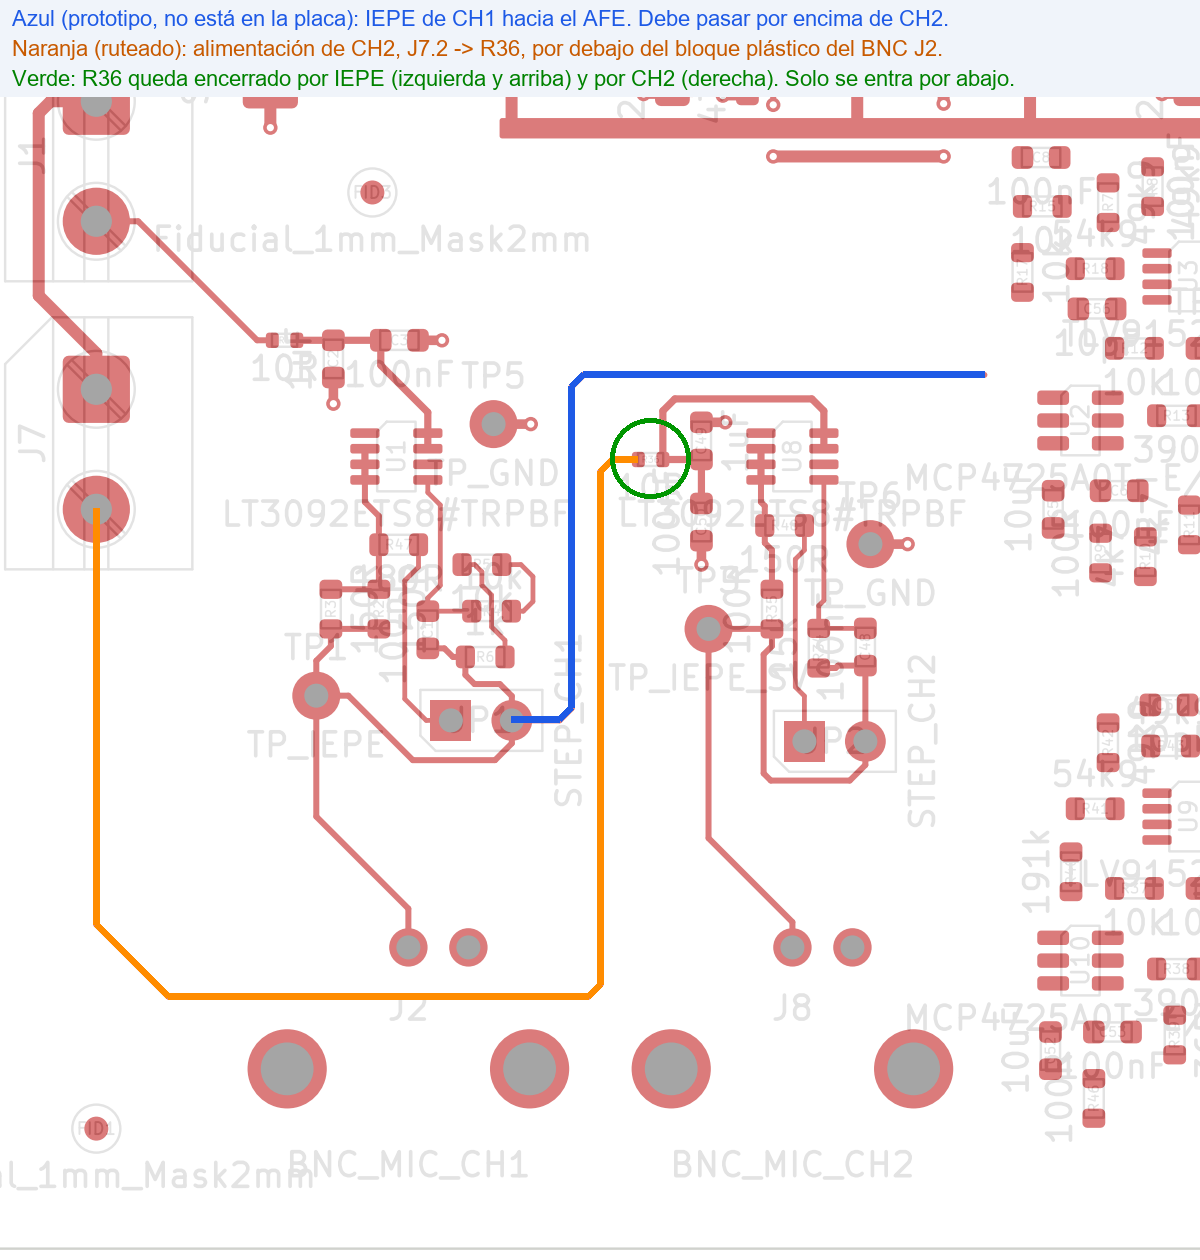
\includegraphics[width=0.75\linewidth]{figuras/bloque3_por_que_bajo_J2.png}
\caption{Bloque 3: por qué la alimentación del canal 2 tuvo que pasar bajo el cuerpo del BNC \net{J2} (prototipo en una
copia de la placa).}
\label{fig:c09-j2}
\end{figure}

\subsection{Bloque 4: el ADC PCM1808}

\begin{itemize}
  \item \textbf{AGND y DGND unidos debajo del integrado}, con una vía al plano, como pide el datasheet
  \doc{SLES177B §10.1.2}. Es el punto donde se tocan la tierra analógica y la digital del convertidor, y conviene que sea
  uno solo y debajo del chip.
  \item \textbf{Desacoplos con su vía:} \net{C17} (\SI{100}{\nano\farad} de VCC) quedó a \SI{0.71}{\milli\meter} del
  pin 3; \net{C11}$\leftrightarrow$\net{C12} y \net{C15}$\leftrightarrow$\net{C16} se intercambiaron para que el
  \SI{100}{\nano\farad} (el que actúa a alta frecuencia) quedara más cerca que el \SI{10}{\micro\farad}.
  \item \textbf{Straps:} \net{MD1} y \net{FMT} son niveles estáticos y quedaban encerrados en \capa{F.Cu} por las
  entradas analógicas; bajan a \capa{In2.Cu}. \net{MD0} pasa por debajo del cuerpo de \net{U4}.
  \item \textbf{Reloj lejos de lo analógico} (\SI{0.5}{\milli\meter}): \net{DOUT} pasa por debajo de \net{R19} gracias a
  que \net{R19} subió \SI{0.1}{\milli\meter}; la salida del oscilador entra a \net{R21} entre sus pads, porque el pad
  GND de \net{Y1} cierra el paso por la izquierda.
\end{itemize}

\subsection{Bloque 5: el AFE de los dos canales}

Es el bloque más delicado: aquí están el nodo \net{SUM}, la cadena de \SI{1}{\mega\ohm} y la realimentación. Todo en
\capa{F.Cu}.
\begin{itemize}
  \item \textbf{Cadena de entrada en columna:} \net{R13} $\to$ \net{R14} $\to$ \net{R16} vertical, y \net{R16.1}
  $\to$ \net{R18.2} pasando centrada entre los pads de \net{R17}.
  \item \textbf{Nodo \net{SUM} mínimo:} \net{R18.1} es el punto de unión; llegan \net{U3.2} (entrada inversora),
  \net{R7.1} (realimentación) y \net{C56.1} (el condensador CF). Cuanto más corto este nodo, menos capacidad parásita
  tiene y menos ruido capta (capítulo~\ref{cap:analog}).
  \item \textbf{La excepción del nodo \net{SUM}:} el enlace \net{C56.1} $\to$ \net{R18.1} no puede entrar por el eje de
  los dos pads con los quiebres fuera de ellos: los pads están a \SI{1.52}{\milli\meter} en $x$ y
  \SI{1.76}{\milli\meter} en $y$, con el otro pad de \net{C56} al lado. Se aceptó el enlace más corto
  (\SI{2.2}{\milli\meter}) con el quiebre a \ang{45} dentro del cobre de los pads. Igual en el canal 2
  (\net{C57.1}--\net{R41.1}).
  \item \textbf{\net{REST_OUT}} sale de \net{U3.1}, sube a \net{R8} y pasa por encima de \net{C7} hasta el punto de
  prueba \net{TP2}. No cabía entre \net{U3.8} y \net{C7} sin cortar el desacoplo; para abrir el paso \net{C7} bajó
  \SI{0.35}{\milli\meter} (queda a \SI{0.975}{\milli\meter} de \net{U3.8}).
  \item \textbf{Canal 2 igual al canal 1:} con la colocación original el canal 2 no salía limpio (el nodo
  \net{R39}--\net{R40} rodeaba el DAC \net{U10}). Se movieron \net{R38}/\net{R39}/\net{R40} a una columna, y \net{C57},
  \net{R43}, \net{TP4}, \net{C54}, \net{R44}, \net{R45} y \net{C55} a las posiciones equivalentes del canal 1. Ahora el
  canal 2 es el canal 1 desplazado \SI{22.5}{\milli\meter}.
\end{itemize}

\begin{figure}[htbp]
\centering
% generado por tikz_zona.py, ventana KiCad (138.5,116.5)-(158.5,139.5) mm, 0.62 cm/mm
\begin{tikzpicture}[line cap=round,line join=round]
\clip (0,0) rectangle (12.400,14.260);
\fill[fondo] (0,0) rectangle (12.400,14.260);
\fill[c24,opacity=0.35] (12.224,14.009) -- (12.232,14.006) -- (12.262,13.984) -- (12.262,13.984) -- (12.264,13.982) -- (12.276,13.946) -- (12.276,13.556) -- (12.273,13.537) -- (12.270,13.529) -- (12.248,13.499) -- (12.246,13.497) -- (12.210,13.485) -- (-10.593,13.485) -- (-10.612,13.488) -- (-10.620,13.491) -- (-10.650,13.513) -- (-10.650,13.513) -- (-10.652,13.515) -- (-10.664,13.551) -- (-10.664,13.941) -- (-10.661,13.960) -- (-10.658,13.968) -- (-10.636,13.998) -- (-10.636,13.999) -- (-10.634,14.000) -- (-10.598,14.012) -- (12.205,14.012) -- cycle;
\filldraw[fill=padfill,draw=paddraw,line width=0.2pt] (1.472,8.262) -- (1.520,8.252) -- (1.560,8.225) -- (1.587,8.185) -- (1.596,8.137) -- (1.596,7.889) -- (1.587,7.842) -- (1.560,7.802) -- (1.520,7.775) -- (1.472,7.766) -- (1.131,7.766) -- (1.084,7.775) -- (1.044,7.802) -- (1.017,7.842) -- (1.008,7.889) -- (1.008,8.137) -- (1.017,8.185) -- (1.044,8.225) -- (1.084,8.252) -- (1.131,8.262) -- cycle;
\filldraw[fill=padfill,draw=paddraw,line width=0.2pt] (1.472,7.238) -- (1.520,7.229) -- (1.560,7.202) -- (1.587,7.162) -- (1.596,7.114) -- (1.596,6.866) -- (1.587,6.819) -- (1.560,6.779) -- (1.520,6.752) -- (1.472,6.742) -- (1.131,6.742) -- (1.084,6.752) -- (1.044,6.779) -- (1.017,6.819) -- (1.008,6.866) -- (1.008,7.114) -- (1.017,7.162) -- (1.044,7.202) -- (1.084,7.229) -- (1.131,7.238) -- cycle;
\filldraw[fill=padfill,draw=paddraw,line width=0.2pt] (3.790,4.666) -- (3.843,4.655) -- (3.888,4.625) -- (3.919,4.579) -- (3.929,4.526) -- (3.929,4.247) -- (3.919,4.194) -- (3.888,4.148) -- (3.843,4.118) -- (3.790,4.108) -- (3.480,4.108) -- (3.426,4.118) -- (3.381,4.148) -- (3.351,4.194) -- (3.340,4.247) -- (3.340,4.526) -- (3.351,4.579) -- (3.381,4.625) -- (3.426,4.655) -- (3.480,4.666) -- cycle;
\filldraw[fill=padfill,draw=paddraw,line width=0.2pt] (3.790,3.705) -- (3.843,3.694) -- (3.888,3.664) -- (3.919,3.618) -- (3.929,3.565) -- (3.929,3.286) -- (3.919,3.233) -- (3.888,3.187) -- (3.843,3.157) -- (3.790,3.147) -- (3.480,3.147) -- (3.426,3.157) -- (3.381,3.187) -- (3.351,3.233) -- (3.340,3.286) -- (3.340,3.565) -- (3.351,3.618) -- (3.381,3.664) -- (3.426,3.694) -- (3.480,3.705) -- cycle;
\filldraw[fill=padfill,draw=paddraw,line width=0.2pt] (1.472,10.273) -- (1.520,10.263) -- (1.560,10.236) -- (1.587,10.196) -- (1.596,10.149) -- (1.596,9.901) -- (1.587,9.853) -- (1.560,9.813) -- (1.520,9.786) -- (1.472,9.777) -- (1.131,9.777) -- (1.084,9.786) -- (1.044,9.813) -- (1.017,9.853) -- (1.008,9.901) -- (1.008,10.149) -- (1.017,10.196) -- (1.044,10.236) -- (1.084,10.263) -- (1.131,10.273) -- cycle;
\filldraw[fill=padfill,draw=paddraw,line width=0.2pt] (1.472,9.250) -- (1.520,9.240) -- (1.560,9.213) -- (1.587,9.173) -- (1.596,9.126) -- (1.596,8.878) -- (1.587,8.830) -- (1.560,8.790) -- (1.520,8.763) -- (1.472,8.754) -- (1.131,8.754) -- (1.084,8.763) -- (1.044,8.790) -- (1.017,8.830) -- (1.008,8.878) -- (1.008,9.126) -- (1.017,9.173) -- (1.044,9.213) -- (1.084,9.240) -- (1.131,9.250) -- cycle;
\filldraw[fill=padfill,draw=paddraw,line width=0.2pt] (7.486,16.120) -- (7.546,16.108) -- (7.596,16.075) -- (7.630,16.024) -- (7.641,15.965) -- (7.641,15.655) -- (7.630,15.596) -- (7.596,15.545) -- (7.546,15.512) -- (7.486,15.500) -- (6.897,15.500) -- (6.838,15.512) -- (6.788,15.545) -- (6.754,15.596) -- (6.742,15.655) -- (6.742,15.965) -- (6.754,16.024) -- (6.788,16.075) -- (6.838,16.108) -- (6.897,16.120) -- cycle;
\filldraw[fill=padfill,draw=paddraw,line width=0.2pt] (7.486,14.942) -- (7.546,14.930) -- (7.596,14.897) -- (7.630,14.846) -- (7.641,14.787) -- (7.641,14.477) -- (7.630,14.418) -- (7.596,14.367) -- (7.546,14.334) -- (7.486,14.322) -- (6.897,14.322) -- (6.838,14.334) -- (6.788,14.367) -- (6.754,14.418) -- (6.742,14.477) -- (6.742,14.787) -- (6.754,14.846) -- (6.788,14.897) -- (6.838,14.930) -- (6.897,14.942) -- cycle;
\filldraw[fill=padfill,draw=paddraw,line width=0.2pt] (13.779,9.540) -- (13.732,9.550) -- (13.692,9.577) -- (13.665,9.617) -- (13.656,9.664) -- (13.656,9.912) -- (13.665,9.960) -- (13.692,10.000) -- (13.732,10.027) -- (13.779,10.036) -- (14.121,10.036) -- (14.168,10.027) -- (14.208,10.000) -- (14.235,9.960) -- (14.244,9.912) -- (14.244,9.664) -- (14.235,9.617) -- (14.208,9.577) -- (14.168,9.550) -- (14.121,9.540) -- cycle;
\filldraw[fill=padfill,draw=paddraw,line width=0.2pt] (13.779,10.563) -- (13.732,10.573) -- (13.692,10.600) -- (13.665,10.640) -- (13.656,10.687) -- (13.656,10.935) -- (13.665,10.983) -- (13.692,11.023) -- (13.732,11.050) -- (13.779,11.059) -- (14.121,11.059) -- (14.168,11.050) -- (14.208,11.023) -- (14.235,10.983) -- (14.244,10.935) -- (14.244,10.687) -- (14.235,10.640) -- (14.208,10.600) -- (14.168,10.573) -- (14.121,10.563) -- cycle;
\filldraw[fill=padfill,draw=paddraw,line width=0.2pt] (4.883,11.067) -- (4.835,11.076) -- (4.795,11.103) -- (4.768,11.144) -- (4.759,11.191) -- (4.759,11.439) -- (4.768,11.486) -- (4.795,11.527) -- (4.835,11.554) -- (4.883,11.563) -- (5.224,11.563) -- (5.271,11.554) -- (5.311,11.527) -- (5.338,11.486) -- (5.348,11.439) -- (5.348,11.191) -- (5.338,11.144) -- (5.311,11.103) -- (5.271,11.076) -- (5.224,11.067) -- cycle;
\filldraw[fill=padfill,draw=paddraw,line width=0.2pt] (4.883,12.090) -- (4.835,12.099) -- (4.795,12.126) -- (4.768,12.167) -- (4.759,12.214) -- (4.759,12.462) -- (4.768,12.509) -- (4.795,12.550) -- (4.835,12.577) -- (4.883,12.586) -- (5.224,12.586) -- (5.271,12.577) -- (5.311,12.550) -- (5.338,12.509) -- (5.348,12.462) -- (5.348,12.214) -- (5.338,12.167) -- (5.311,12.126) -- (5.271,12.099) -- (5.224,12.090) -- cycle;
\filldraw[fill=padfill,draw=paddraw,line width=0.2pt] (7.056,8.219) -- (7.067,8.272) -- (7.097,8.318) -- (7.142,8.348) -- (7.196,8.359) -- (7.475,8.359) -- (7.528,8.348) -- (7.574,8.318) -- (7.604,8.272) -- (7.614,8.219) -- (7.614,7.909) -- (7.604,7.856) -- (7.574,7.810) -- (7.528,7.780) -- (7.475,7.770) -- (7.196,7.770) -- (7.142,7.780) -- (7.097,7.810) -- (7.067,7.856) -- (7.056,7.909) -- cycle;
\filldraw[fill=padfill,draw=paddraw,line width=0.2pt] (8.017,8.219) -- (8.028,8.272) -- (8.058,8.318) -- (8.103,8.348) -- (8.157,8.359) -- (8.436,8.359) -- (8.489,8.348) -- (8.535,8.318) -- (8.565,8.272) -- (8.575,8.219) -- (8.575,7.909) -- (8.565,7.856) -- (8.535,7.810) -- (8.489,7.780) -- (8.436,7.770) -- (8.157,7.770) -- (8.103,7.780) -- (8.058,7.810) -- (8.028,7.856) -- (8.017,7.909) -- cycle;
\filldraw[fill=padfill,draw=paddraw,line width=0.2pt] (3.224,6.882) -- (3.231,6.918) -- (3.251,6.948) -- (3.281,6.968) -- (3.317,6.975) -- (3.953,6.975) -- (3.988,6.968) -- (4.018,6.948) -- (4.038,6.918) -- (4.046,6.882) -- (4.046,6.696) -- (4.038,6.660) -- (4.018,6.630) -- (3.988,6.610) -- (3.953,6.603) -- (3.317,6.603) -- (3.281,6.610) -- (3.251,6.630) -- (3.231,6.660) -- (3.224,6.696) -- cycle;
\filldraw[fill=padfill,draw=paddraw,line width=0.2pt] (3.224,6.293) -- (3.231,6.329) -- (3.251,6.359) -- (3.281,6.379) -- (3.317,6.386) -- (3.953,6.386) -- (3.988,6.379) -- (4.018,6.359) -- (4.038,6.329) -- (4.046,6.293) -- (4.046,6.107) -- (4.038,6.071) -- (4.018,6.041) -- (3.988,6.021) -- (3.953,6.014) -- (3.317,6.014) -- (3.281,6.021) -- (3.251,6.041) -- (3.231,6.071) -- (3.224,6.107) -- cycle;
\filldraw[fill=padfill,draw=paddraw,line width=0.2pt] (3.224,5.704) -- (3.231,5.740) -- (3.251,5.770) -- (3.281,5.790) -- (3.317,5.797) -- (3.953,5.797) -- (3.988,5.790) -- (4.018,5.770) -- (4.038,5.740) -- (4.046,5.704) -- (4.046,5.518) -- (4.038,5.482) -- (4.018,5.452) -- (3.988,5.432) -- (3.953,5.425) -- (3.317,5.425) -- (3.281,5.432) -- (3.251,5.452) -- (3.231,5.482) -- (3.224,5.518) -- cycle;
\filldraw[fill=padfill,draw=paddraw,line width=0.2pt] (4.634,5.704) -- (4.642,5.740) -- (4.662,5.770) -- (4.692,5.790) -- (4.728,5.797) -- (5.363,5.797) -- (5.399,5.790) -- (5.429,5.770) -- (5.449,5.740) -- (5.456,5.704) -- (5.456,5.518) -- (5.449,5.482) -- (5.429,5.452) -- (5.399,5.432) -- (5.363,5.425) -- (4.728,5.425) -- (4.692,5.432) -- (4.662,5.452) -- (4.642,5.482) -- (4.634,5.518) -- cycle;
\filldraw[fill=padfill,draw=paddraw,line width=0.2pt] (4.634,6.293) -- (4.642,6.329) -- (4.662,6.359) -- (4.692,6.379) -- (4.728,6.386) -- (5.363,6.386) -- (5.399,6.379) -- (5.429,6.359) -- (5.449,6.329) -- (5.456,6.293) -- (5.456,6.107) -- (5.449,6.071) -- (5.429,6.041) -- (5.399,6.021) -- (5.363,6.014) -- (4.728,6.014) -- (4.692,6.021) -- (4.662,6.041) -- (4.642,6.071) -- (4.634,6.107) -- cycle;
\filldraw[fill=padfill,draw=paddraw,line width=0.2pt] (4.634,6.882) -- (4.642,6.918) -- (4.662,6.948) -- (4.692,6.968) -- (4.728,6.975) -- (5.363,6.975) -- (5.399,6.968) -- (5.429,6.948) -- (5.449,6.918) -- (5.456,6.882) -- (5.456,6.696) -- (5.449,6.660) -- (5.429,6.630) -- (5.399,6.610) -- (5.363,6.603) -- (4.728,6.603) -- (4.692,6.610) -- (4.662,6.630) -- (4.642,6.660) -- (4.634,6.696) -- cycle;
\filldraw[fill=padfill,draw=paddraw,line width=0.2pt] (4.883,-1.860) -- (4.835,-1.851) -- (4.795,-1.824) -- (4.768,-1.783) -- (4.759,-1.736) -- (4.759,-1.488) -- (4.768,-1.441) -- (4.795,-1.400) -- (4.835,-1.373) -- (4.883,-1.364) -- (5.224,-1.364) -- (5.271,-1.373) -- (5.311,-1.400) -- (5.338,-1.441) -- (5.348,-1.488) -- (5.348,-1.736) -- (5.338,-1.783) -- (5.311,-1.824) -- (5.271,-1.851) -- (5.224,-1.860) -- cycle;
\filldraw[fill=padfill,draw=paddraw,line width=0.2pt] (4.976,8.235) -- (4.985,8.282) -- (5.012,8.322) -- (5.052,8.349) -- (5.099,8.359) -- (5.348,8.359) -- (5.395,8.349) -- (5.435,8.322) -- (5.462,8.282) -- (5.471,8.235) -- (5.471,7.894) -- (5.462,7.846) -- (5.435,7.806) -- (5.395,7.779) -- (5.348,7.770) -- (5.099,7.770) -- (5.052,7.779) -- (5.012,7.806) -- (4.985,7.846) -- (4.976,7.894) -- cycle;
\filldraw[fill=padfill,draw=paddraw,line width=0.2pt] (5.999,8.235) -- (6.008,8.282) -- (6.035,8.322) -- (6.075,8.349) -- (6.122,8.359) -- (6.371,8.359) -- (6.418,8.349) -- (6.458,8.322) -- (6.485,8.282) -- (6.494,8.235) -- (6.494,7.894) -- (6.485,7.846) -- (6.458,7.806) -- (6.418,7.779) -- (6.371,7.770) -- (6.122,7.770) -- (6.075,7.779) -- (6.035,7.806) -- (6.008,7.846) -- (5.999,7.894) -- cycle;
\filldraw[fill=padfill,draw=paddraw,line width=0.2pt] (10.305,10.585) -- (10.281,10.705) -- (10.235,10.817) -- (10.167,10.918) -- (10.081,11.004) -- (9.980,11.071) -- (9.868,11.118) -- (9.749,11.142) -- (9.627,11.142) -- (9.508,11.118) -- (9.396,11.071) -- (9.295,11.004) -- (9.209,10.918) -- (9.141,10.817) -- (9.095,10.705) -- (9.071,10.585) -- (9.071,10.464) -- (9.095,10.345) -- (9.141,10.232) -- (9.209,10.131) -- (9.295,10.045) -- (9.396,9.978) -- (9.508,9.931) -- (9.627,9.908) -- (9.749,9.908) -- (9.868,9.931) -- (9.980,9.978) -- (10.081,10.045) -- (10.167,10.131) -- (10.235,10.232) -- (10.281,10.345) -- (10.305,10.464) -- (10.305,10.585) -- cycle;
\fill[white] (9.688,10.525) circle (0.310);
\filldraw[fill=padfill,draw=paddraw,line width=0.2pt] (2.672,9.265) -- (2.624,9.275) -- (2.584,9.301) -- (2.557,9.342) -- (2.548,9.389) -- (2.548,9.637) -- (2.557,9.685) -- (2.584,9.725) -- (2.624,9.752) -- (2.672,9.761) -- (3.013,9.761) -- (3.060,9.752) -- (3.100,9.725) -- (3.127,9.685) -- (3.137,9.637) -- (3.137,9.389) -- (3.127,9.342) -- (3.100,9.301) -- (3.060,9.275) -- (3.013,9.265) -- cycle;
\filldraw[fill=padfill,draw=paddraw,line width=0.2pt] (2.672,10.288) -- (2.624,10.298) -- (2.584,10.324) -- (2.557,10.365) -- (2.548,10.412) -- (2.548,10.660) -- (2.557,10.708) -- (2.584,10.748) -- (2.624,10.775) -- (2.672,10.784) -- (3.013,10.784) -- (3.060,10.775) -- (3.100,10.748) -- (3.127,10.708) -- (3.137,10.660) -- (3.137,10.412) -- (3.127,10.365) -- (3.100,10.324) -- (3.060,10.298) -- (3.013,10.288) -- cycle;
\filldraw[fill=padfill,draw=paddraw,line width=0.2pt] (5.030,3.537) -- (5.077,3.527) -- (5.117,3.500) -- (5.144,3.460) -- (5.154,3.413) -- (5.154,3.165) -- (5.144,3.117) -- (5.117,3.077) -- (5.077,3.050) -- (5.030,3.041) -- (4.689,3.041) -- (4.641,3.050) -- (4.601,3.077) -- (4.574,3.117) -- (4.565,3.165) -- (4.565,3.413) -- (4.574,3.460) -- (4.601,3.500) -- (4.641,3.527) -- (4.689,3.537) -- cycle;
\filldraw[fill=padfill,draw=paddraw,line width=0.2pt] (5.030,2.514) -- (5.077,2.504) -- (5.117,2.477) -- (5.144,2.437) -- (5.154,2.390) -- (5.154,2.142) -- (5.144,2.094) -- (5.117,2.054) -- (5.077,2.027) -- (5.030,2.018) -- (4.689,2.018) -- (4.641,2.027) -- (4.601,2.054) -- (4.574,2.094) -- (4.565,2.142) -- (4.565,2.390) -- (4.574,2.437) -- (4.601,2.477) -- (4.641,2.504) -- (4.689,2.514) -- cycle;
\filldraw[fill=padfill,draw=paddraw,line width=0.2pt] (14.027,3.503) -- (14.017,3.450) -- (13.987,3.404) -- (13.941,3.374) -- (13.888,3.364) -- (13.609,3.364) -- (13.556,3.374) -- (13.510,3.404) -- (13.480,3.450) -- (13.469,3.503) -- (13.469,3.813) -- (13.480,3.866) -- (13.510,3.912) -- (13.556,3.942) -- (13.609,3.953) -- (13.888,3.953) -- (13.941,3.942) -- (13.987,3.912) -- (14.017,3.866) -- (14.027,3.813) -- cycle;
\filldraw[fill=padfill,draw=paddraw,line width=0.2pt] (6.033,-1.434) -- (5.986,-1.424) -- (5.946,-1.398) -- (5.919,-1.357) -- (5.909,-1.310) -- (5.909,-1.062) -- (5.919,-1.014) -- (5.946,-0.974) -- (5.986,-0.947) -- (6.033,-0.938) -- (6.374,-0.938) -- (6.422,-0.947) -- (6.462,-0.974) -- (6.489,-1.014) -- (6.498,-1.062) -- (6.498,-1.310) -- (6.489,-1.357) -- (6.462,-1.398) -- (6.422,-1.424) -- (6.374,-1.434) -- cycle;
\filldraw[fill=padfill,draw=paddraw,line width=0.2pt] (13.082,1.627) -- (13.135,1.617) -- (13.181,1.587) -- (13.211,1.541) -- (13.221,1.488) -- (13.221,1.209) -- (13.211,1.156) -- (13.181,1.110) -- (13.135,1.080) -- (13.082,1.069) -- (12.772,1.069) -- (12.719,1.080) -- (12.673,1.110) -- (12.643,1.156) -- (12.633,1.209) -- (12.633,1.488) -- (12.643,1.541) -- (12.673,1.587) -- (12.719,1.617) -- (12.772,1.627) -- cycle;
\filldraw[fill=padfill,draw=paddraw,line width=0.2pt] (13.082,0.666) -- (13.135,0.656) -- (13.181,0.626) -- (13.211,0.580) -- (13.221,0.527) -- (13.221,0.248) -- (13.211,0.195) -- (13.181,0.149) -- (13.135,0.119) -- (13.082,0.109) -- (12.772,0.109) -- (12.719,0.119) -- (12.673,0.149) -- (12.643,0.195) -- (12.633,0.248) -- (12.633,0.527) -- (12.643,0.580) -- (12.673,0.626) -- (12.719,0.656) -- (12.772,0.666) -- cycle;
\filldraw[fill=padfill,draw=paddraw,line width=0.2pt] (2.687,-0.705) -- (2.698,-0.652) -- (2.728,-0.607) -- (2.773,-0.576) -- (2.827,-0.566) -- (3.106,-0.566) -- (3.159,-0.576) -- (3.204,-0.607) -- (3.235,-0.652) -- (3.245,-0.705) -- (3.245,-1.015) -- (3.235,-1.069) -- (3.204,-1.114) -- (3.159,-1.144) -- (3.106,-1.155) -- (2.827,-1.155) -- (2.773,-1.144) -- (2.728,-1.114) -- (2.698,-1.069) -- (2.687,-1.015) -- cycle;
\filldraw[fill=padfill,draw=paddraw,line width=0.2pt] (3.648,-0.705) -- (3.659,-0.652) -- (3.689,-0.607) -- (3.734,-0.576) -- (3.788,-0.566) -- (4.067,-0.566) -- (4.120,-0.576) -- (4.165,-0.607) -- (4.196,-0.652) -- (4.206,-0.705) -- (4.206,-1.015) -- (4.196,-1.069) -- (4.165,-1.114) -- (4.120,-1.144) -- (4.067,-1.155) -- (3.788,-1.155) -- (3.734,-1.144) -- (3.689,-1.114) -- (3.659,-1.069) -- (3.648,-1.015) -- cycle;
\filldraw[fill=padfill,draw=paddraw,line width=0.2pt] (4.580,4.541) -- (4.591,4.595) -- (4.621,4.640) -- (4.666,4.670) -- (4.720,4.681) -- (4.999,4.681) -- (5.052,4.670) -- (5.097,4.640) -- (5.128,4.595) -- (5.138,4.541) -- (5.138,4.231) -- (5.128,4.178) -- (5.097,4.133) -- (5.052,4.103) -- (4.999,4.092) -- (4.720,4.092) -- (4.666,4.103) -- (4.621,4.133) -- (4.591,4.178) -- (4.580,4.231) -- cycle;
\filldraw[fill=padfill,draw=paddraw,line width=0.2pt] (5.541,4.541) -- (5.552,4.595) -- (5.582,4.640) -- (5.627,4.670) -- (5.681,4.681) -- (5.960,4.681) -- (6.013,4.670) -- (6.058,4.640) -- (6.089,4.595) -- (6.099,4.541) -- (6.099,4.231) -- (6.089,4.178) -- (6.058,4.133) -- (6.013,4.103) -- (5.960,4.092) -- (5.681,4.092) -- (5.627,4.103) -- (5.582,4.133) -- (5.552,4.178) -- (5.541,4.231) -- cycle;
\filldraw[fill=padfill,draw=paddraw,line width=0.2pt] (2.594,11.900) -- (2.604,11.948) -- (2.631,11.988) -- (2.671,12.015) -- (2.718,12.024) -- (2.966,12.024) -- (3.014,12.015) -- (3.054,11.988) -- (3.081,11.948) -- (3.090,11.900) -- (3.090,11.559) -- (3.081,11.512) -- (3.054,11.471) -- (3.014,11.445) -- (2.966,11.435) -- (2.718,11.435) -- (2.671,11.445) -- (2.631,11.471) -- (2.604,11.512) -- (2.594,11.559) -- cycle;
\filldraw[fill=padfill,draw=paddraw,line width=0.2pt] (3.617,11.900) -- (3.627,11.948) -- (3.654,11.988) -- (3.694,12.015) -- (3.741,12.024) -- (3.989,12.024) -- (4.037,12.015) -- (4.077,11.988) -- (4.104,11.948) -- (4.113,11.900) -- (4.113,11.559) -- (4.104,11.512) -- (4.077,11.471) -- (4.037,11.445) -- (3.989,11.435) -- (3.741,11.435) -- (3.694,11.445) -- (3.654,11.471) -- (3.627,11.512) -- (3.617,11.559) -- cycle;
\filldraw[fill=padfill,draw=paddraw,line width=0.2pt] (5.940,10.587) -- (5.944,10.610) -- (5.958,10.630) -- (5.978,10.644) -- (6.002,10.648) -- (6.634,10.648) -- (6.658,10.644) -- (6.678,10.630) -- (6.691,10.610) -- (6.696,10.587) -- (6.696,10.463) -- (6.691,10.439) -- (6.678,10.419) -- (6.658,10.405) -- (6.634,10.401) -- (6.002,10.401) -- (5.978,10.405) -- (5.958,10.419) -- (5.944,10.439) -- (5.940,10.463) -- cycle;
\filldraw[fill=padfill,draw=paddraw,line width=0.2pt] (5.940,10.183) -- (5.944,10.207) -- (5.958,10.227) -- (5.978,10.241) -- (6.002,10.246) -- (6.634,10.246) -- (6.658,10.241) -- (6.678,10.227) -- (6.691,10.207) -- (6.696,10.183) -- (6.696,10.059) -- (6.691,10.036) -- (6.678,10.016) -- (6.658,10.002) -- (6.634,9.998) -- (6.002,9.998) -- (5.978,10.002) -- (5.958,10.016) -- (5.944,10.036) -- (5.940,10.059) -- cycle;
\filldraw[fill=padfill,draw=paddraw,line width=0.2pt] (5.940,9.781) -- (5.944,9.804) -- (5.958,9.824) -- (5.978,9.838) -- (6.002,9.842) -- (6.634,9.842) -- (6.658,9.838) -- (6.678,9.824) -- (6.691,9.804) -- (6.696,9.781) -- (6.696,9.657) -- (6.691,9.633) -- (6.678,9.613) -- (6.658,9.599) -- (6.634,9.594) -- (6.002,9.594) -- (5.978,9.599) -- (5.958,9.613) -- (5.944,9.633) -- (5.940,9.657) -- cycle;
\filldraw[fill=padfill,draw=paddraw,line width=0.2pt] (5.940,9.377) -- (5.944,9.401) -- (5.958,9.421) -- (5.978,9.435) -- (6.002,9.439) -- (6.634,9.439) -- (6.658,9.435) -- (6.678,9.421) -- (6.691,9.401) -- (6.696,9.377) -- (6.696,9.253) -- (6.691,9.230) -- (6.678,9.210) -- (6.658,9.196) -- (6.634,9.192) -- (6.002,9.192) -- (5.978,9.196) -- (5.958,9.210) -- (5.944,9.230) -- (5.940,9.253) -- cycle;
\filldraw[fill=padfill,draw=paddraw,line width=0.2pt] (7.564,9.377) -- (7.569,9.401) -- (7.582,9.421) -- (7.602,9.435) -- (7.626,9.439) -- (8.258,9.439) -- (8.282,9.435) -- (8.302,9.421) -- (8.316,9.401) -- (8.320,9.377) -- (8.320,9.253) -- (8.316,9.230) -- (8.302,9.210) -- (8.282,9.196) -- (8.258,9.192) -- (7.626,9.192) -- (7.602,9.196) -- (7.582,9.210) -- (7.569,9.230) -- (7.564,9.253) -- cycle;
\filldraw[fill=padfill,draw=paddraw,line width=0.2pt] (7.564,9.781) -- (7.569,9.804) -- (7.582,9.824) -- (7.602,9.838) -- (7.626,9.842) -- (8.258,9.842) -- (8.282,9.838) -- (8.302,9.824) -- (8.316,9.804) -- (8.320,9.781) -- (8.320,9.657) -- (8.316,9.633) -- (8.302,9.613) -- (8.282,9.599) -- (8.258,9.594) -- (7.626,9.594) -- (7.602,9.599) -- (7.582,9.613) -- (7.569,9.633) -- (7.564,9.657) -- cycle;
\filldraw[fill=padfill,draw=paddraw,line width=0.2pt] (7.564,10.183) -- (7.569,10.207) -- (7.582,10.227) -- (7.602,10.241) -- (7.626,10.246) -- (8.258,10.246) -- (8.282,10.241) -- (8.302,10.227) -- (8.316,10.207) -- (8.320,10.183) -- (8.320,10.059) -- (8.316,10.036) -- (8.302,10.016) -- (8.282,10.002) -- (8.258,9.998) -- (7.626,9.998) -- (7.602,10.002) -- (7.582,10.016) -- (7.569,10.036) -- (7.564,10.059) -- cycle;
\filldraw[fill=padfill,draw=paddraw,line width=0.2pt] (7.564,10.587) -- (7.569,10.610) -- (7.582,10.630) -- (7.602,10.644) -- (7.626,10.648) -- (8.258,10.648) -- (8.282,10.644) -- (8.302,10.630) -- (8.316,10.610) -- (8.320,10.587) -- (8.320,10.463) -- (8.316,10.439) -- (8.302,10.419) -- (8.282,10.405) -- (8.258,10.401) -- (7.626,10.401) -- (7.602,10.405) -- (7.582,10.419) -- (7.569,10.439) -- (7.564,10.463) -- cycle;
\filldraw[fill=padfill,draw=paddraw,line width=0.2pt] (4.008,9.188) -- (4.019,9.242) -- (4.049,9.287) -- (4.094,9.317) -- (4.148,9.328) -- (4.427,9.328) -- (4.480,9.317) -- (4.525,9.287) -- (4.556,9.242) -- (4.566,9.188) -- (4.566,8.878) -- (4.556,8.825) -- (4.525,8.780) -- (4.480,8.750) -- (4.427,8.739) -- (4.148,8.739) -- (4.094,8.750) -- (4.049,8.780) -- (4.019,8.825) -- (4.008,8.878) -- cycle;
\filldraw[fill=padfill,draw=paddraw,line width=0.2pt] (4.969,9.188) -- (4.980,9.242) -- (5.010,9.287) -- (5.055,9.317) -- (5.109,9.328) -- (5.388,9.328) -- (5.441,9.317) -- (5.486,9.287) -- (5.517,9.242) -- (5.527,9.188) -- (5.527,8.878) -- (5.517,8.825) -- (5.486,8.780) -- (5.441,8.750) -- (5.388,8.739) -- (5.109,8.739) -- (5.055,8.750) -- (5.010,8.780) -- (4.980,8.825) -- (4.969,8.878) -- cycle;
\filldraw[fill=padfill,draw=paddraw,line width=0.2pt] (14.467,1.431) -- (14.456,1.377) -- (14.426,1.332) -- (14.380,1.302) -- (14.327,1.291) -- (14.048,1.291) -- (13.995,1.302) -- (13.949,1.332) -- (13.919,1.377) -- (13.909,1.431) -- (13.909,1.741) -- (13.919,1.794) -- (13.949,1.839) -- (13.995,1.870) -- (14.048,1.880) -- (14.327,1.880) -- (14.380,1.870) -- (14.426,1.839) -- (14.456,1.794) -- (14.467,1.741) -- cycle;
\filldraw[fill=padfill,draw=paddraw,line width=0.2pt] (6.033,11.481) -- (5.986,11.491) -- (5.946,11.518) -- (5.919,11.558) -- (5.909,11.605) -- (5.909,11.853) -- (5.919,11.901) -- (5.946,11.941) -- (5.986,11.968) -- (6.033,11.977) -- (6.374,11.977) -- (6.422,11.968) -- (6.462,11.941) -- (6.489,11.901) -- (6.498,11.853) -- (6.498,11.605) -- (6.489,11.558) -- (6.462,11.518) -- (6.422,11.491) -- (6.374,11.481) -- cycle;
\filldraw[fill=padfill,draw=paddraw,line width=0.2pt] (6.033,12.504) -- (5.986,12.514) -- (5.946,12.541) -- (5.919,12.581) -- (5.909,12.628) -- (5.909,12.876) -- (5.919,12.924) -- (5.946,12.964) -- (5.986,12.991) -- (6.033,13.000) -- (6.374,13.000) -- (6.422,12.991) -- (6.462,12.964) -- (6.489,12.924) -- (6.498,12.876) -- (6.498,12.628) -- (6.489,12.581) -- (6.462,12.541) -- (6.422,12.514) -- (6.374,12.504) -- cycle;
\filldraw[fill=padfill,draw=paddraw,line width=0.2pt] (7.990,-1.178) -- (8.044,-1.189) -- (8.089,-1.219) -- (8.119,-1.264) -- (8.130,-1.317) -- (8.130,-1.596) -- (8.119,-1.650) -- (8.089,-1.695) -- (8.044,-1.725) -- (7.990,-1.736) -- (7.680,-1.736) -- (7.627,-1.725) -- (7.582,-1.695) -- (7.551,-1.650) -- (7.541,-1.596) -- (7.541,-1.317) -- (7.551,-1.264) -- (7.582,-1.219) -- (7.627,-1.189) -- (7.680,-1.178) -- cycle;
\filldraw[fill=padfill,draw=paddraw,line width=0.2pt] (13.221,5.681) -- (13.168,5.691) -- (13.123,5.722) -- (13.092,5.767) -- (13.082,5.820) -- (13.082,6.099) -- (13.092,6.153) -- (13.123,6.198) -- (13.168,6.228) -- (13.221,6.239) -- (13.531,6.239) -- (13.585,6.228) -- (13.630,6.198) -- (13.660,6.153) -- (13.671,6.099) -- (13.671,5.820) -- (13.660,5.767) -- (13.630,5.722) -- (13.585,5.691) -- (13.531,5.681) -- cycle;
\filldraw[fill=padfill,draw=paddraw,line width=0.2pt] (13.221,6.642) -- (13.168,6.652) -- (13.123,6.683) -- (13.092,6.728) -- (13.082,6.781) -- (13.082,7.060) -- (13.092,7.114) -- (13.123,7.159) -- (13.168,7.189) -- (13.221,7.200) -- (13.531,7.200) -- (13.585,7.189) -- (13.630,7.159) -- (13.660,7.114) -- (13.671,7.060) -- (13.671,6.781) -- (13.660,6.728) -- (13.630,6.683) -- (13.585,6.652) -- (13.531,6.642) -- cycle;
\filldraw[fill=padfill,draw=paddraw,line width=0.2pt] (5.479,9.951) -- (5.470,9.904) -- (5.443,9.863) -- (5.403,9.836) -- (5.355,9.827) -- (5.107,9.827) -- (5.060,9.836) -- (5.020,9.863) -- (4.993,9.904) -- (4.983,9.951) -- (4.983,10.292) -- (4.993,10.339) -- (5.020,10.380) -- (5.060,10.407) -- (5.107,10.416) -- (5.355,10.416) -- (5.403,10.407) -- (5.443,10.380) -- (5.470,10.339) -- (5.479,10.292) -- cycle;
\filldraw[fill=padfill,draw=paddraw,line width=0.2pt] (4.456,9.951) -- (4.447,9.904) -- (4.420,9.863) -- (4.380,9.836) -- (4.332,9.827) -- (4.084,9.827) -- (4.037,9.836) -- (3.997,9.863) -- (3.970,9.904) -- (3.960,9.951) -- (3.960,10.292) -- (3.970,10.339) -- (3.997,10.380) -- (4.037,10.407) -- (4.084,10.416) -- (4.332,10.416) -- (4.380,10.407) -- (4.420,10.380) -- (4.447,10.339) -- (4.456,10.292) -- cycle;
\filldraw[fill=padfill,draw=paddraw,line width=0.2pt] (1.472,6.246) -- (1.520,6.237) -- (1.560,6.210) -- (1.587,6.170) -- (1.596,6.122) -- (1.596,5.874) -- (1.587,5.827) -- (1.560,5.787) -- (1.520,5.760) -- (1.472,5.751) -- (1.131,5.751) -- (1.084,5.760) -- (1.044,5.787) -- (1.017,5.827) -- (1.008,5.874) -- (1.008,6.122) -- (1.017,6.170) -- (1.044,6.210) -- (1.084,6.237) -- (1.131,6.246) -- cycle;
\filldraw[fill=padfill,draw=paddraw,line width=0.2pt] (1.472,5.224) -- (1.520,5.214) -- (1.560,5.187) -- (1.587,5.147) -- (1.596,5.099) -- (1.596,4.851) -- (1.587,4.804) -- (1.560,4.764) -- (1.520,4.737) -- (1.472,4.728) -- (1.131,4.728) -- (1.084,4.737) -- (1.044,4.764) -- (1.017,4.804) -- (1.008,4.851) -- (1.008,5.099) -- (1.017,5.147) -- (1.044,5.187) -- (1.084,5.214) -- (1.131,5.224) -- cycle;
\filldraw[fill=padfill,draw=paddraw,line width=0.2pt] (12.679,9.556) -- (12.726,9.546) -- (12.767,9.519) -- (12.794,9.479) -- (12.803,9.432) -- (12.803,9.184) -- (12.794,9.136) -- (12.767,9.096) -- (12.726,9.069) -- (12.679,9.060) -- (12.338,9.060) -- (12.291,9.069) -- (12.250,9.096) -- (12.223,9.136) -- (12.214,9.184) -- (12.214,9.432) -- (12.223,9.479) -- (12.250,9.519) -- (12.291,9.546) -- (12.338,9.556) -- cycle;
\filldraw[fill=padfill,draw=paddraw,line width=0.2pt] (12.679,8.533) -- (12.726,8.523) -- (12.767,8.496) -- (12.794,8.456) -- (12.803,8.409) -- (12.803,8.161) -- (12.794,8.113) -- (12.767,8.073) -- (12.726,8.046) -- (12.679,8.037) -- (12.338,8.037) -- (12.291,8.046) -- (12.250,8.073) -- (12.223,8.113) -- (12.214,8.161) -- (12.214,8.409) -- (12.223,8.456) -- (12.250,8.496) -- (12.291,8.523) -- (12.338,8.533) -- cycle;
\filldraw[fill=padfill,draw=paddraw,line width=0.2pt] (7.990,12.772) -- (8.044,12.761) -- (8.089,12.731) -- (8.119,12.686) -- (8.130,12.633) -- (8.130,12.353) -- (8.119,12.300) -- (8.089,12.255) -- (8.044,12.225) -- (7.990,12.214) -- (7.680,12.214) -- (7.627,12.225) -- (7.582,12.255) -- (7.551,12.300) -- (7.541,12.353) -- (7.541,12.633) -- (7.551,12.686) -- (7.582,12.731) -- (7.627,12.761) -- (7.680,12.772) -- cycle;
\filldraw[fill=padfill,draw=paddraw,line width=0.2pt] (7.990,11.811) -- (8.044,11.800) -- (8.089,11.770) -- (8.119,11.725) -- (8.130,11.672) -- (8.130,11.393) -- (8.119,11.339) -- (8.089,11.294) -- (8.044,11.264) -- (7.990,11.253) -- (7.680,11.253) -- (7.627,11.264) -- (7.582,11.294) -- (7.551,11.339) -- (7.541,11.393) -- (7.541,11.672) -- (7.551,11.725) -- (7.582,11.770) -- (7.627,11.800) -- (7.680,11.811) -- cycle;
\filldraw[fill=padfill,draw=paddraw,line width=0.2pt] (9.300,15.862) -- (9.347,15.852) -- (9.388,15.826) -- (9.415,15.785) -- (9.424,15.738) -- (9.424,15.490) -- (9.415,15.442) -- (9.388,15.402) -- (9.347,15.375) -- (9.300,15.366) -- (8.959,15.366) -- (8.912,15.375) -- (8.871,15.402) -- (8.844,15.442) -- (8.835,15.490) -- (8.835,15.738) -- (8.844,15.785) -- (8.871,15.826) -- (8.912,15.852) -- (8.959,15.862) -- cycle;
\filldraw[fill=padfill,draw=paddraw,line width=0.2pt] (9.300,14.839) -- (9.347,14.829) -- (9.388,14.803) -- (9.415,14.762) -- (9.424,14.715) -- (9.424,14.467) -- (9.415,14.419) -- (9.388,14.379) -- (9.347,14.352) -- (9.300,14.343) -- (8.959,14.343) -- (8.912,14.352) -- (8.871,14.379) -- (8.844,14.419) -- (8.835,14.467) -- (8.835,14.715) -- (8.844,14.762) -- (8.871,14.803) -- (8.912,14.829) -- (8.959,14.839) -- cycle;
\filldraw[fill=padfill,draw=paddraw,line width=0.2pt] (2.563,13.148) -- (2.574,13.201) -- (2.604,13.247) -- (2.649,13.277) -- (2.703,13.287) -- (2.982,13.287) -- (3.035,13.277) -- (3.080,13.247) -- (3.111,13.201) -- (3.121,13.148) -- (3.121,12.838) -- (3.111,12.784) -- (3.080,12.739) -- (3.035,12.709) -- (2.982,12.698) -- (2.703,12.698) -- (2.649,12.709) -- (2.604,12.739) -- (2.574,12.784) -- (2.563,12.838) -- cycle;
\filldraw[fill=padfill,draw=paddraw,line width=0.2pt] (3.524,13.148) -- (3.535,13.201) -- (3.565,13.247) -- (3.610,13.277) -- (3.664,13.287) -- (3.943,13.287) -- (3.996,13.277) -- (4.041,13.247) -- (4.072,13.201) -- (4.082,13.148) -- (4.082,12.838) -- (4.072,12.784) -- (4.041,12.739) -- (3.996,12.709) -- (3.943,12.698) -- (3.664,12.698) -- (3.610,12.709) -- (3.565,12.739) -- (3.535,12.784) -- (3.524,12.838) -- cycle;
\filldraw[fill=padfill,draw=paddraw,line width=0.2pt] (-1.061,1.110) -- (-1.008,1.099) -- (-0.962,1.069) -- (-0.932,1.023) -- (-0.921,0.970) -- (-0.921,0.691) -- (-0.932,0.638) -- (-0.962,0.592) -- (-1.008,0.562) -- (-1.061,0.552) -- (-1.371,0.552) -- (-1.424,0.562) -- (-1.470,0.592) -- (-1.500,0.638) -- (-1.510,0.691) -- (-1.510,0.970) -- (-1.500,1.023) -- (-1.470,1.069) -- (-1.424,1.099) -- (-1.371,1.110) -- cycle;
\filldraw[fill=padfill,draw=paddraw,line width=0.2pt] (-1.061,0.149) -- (-1.008,0.138) -- (-0.962,0.108) -- (-0.932,0.062) -- (-0.921,0.009) -- (-0.921,-0.270) -- (-0.932,-0.323) -- (-0.962,-0.369) -- (-1.008,-0.399) -- (-1.061,-0.409) -- (-1.371,-0.409) -- (-1.424,-0.399) -- (-1.470,-0.369) -- (-1.500,-0.323) -- (-1.510,-0.270) -- (-1.510,0.009) -- (-1.500,0.062) -- (-1.470,0.108) -- (-1.424,0.138) -- (-1.371,0.149) -- cycle;
\filldraw[fill=padfill,draw=paddraw,line width=0.2pt] (12.664,11.577) -- (12.717,11.566) -- (12.762,11.536) -- (12.792,11.491) -- (12.803,11.437) -- (12.803,11.158) -- (12.792,11.105) -- (12.762,11.060) -- (12.717,11.030) -- (12.664,11.019) -- (12.354,11.019) -- (12.300,11.030) -- (12.255,11.060) -- (12.225,11.105) -- (12.214,11.158) -- (12.214,11.437) -- (12.225,11.491) -- (12.255,11.536) -- (12.300,11.566) -- (12.354,11.577) -- cycle;
\filldraw[fill=padfill,draw=paddraw,line width=0.2pt] (12.664,10.616) -- (12.717,10.605) -- (12.762,10.575) -- (12.792,10.530) -- (12.803,10.476) -- (12.803,10.197) -- (12.792,10.144) -- (12.762,10.099) -- (12.717,10.069) -- (12.664,10.058) -- (12.354,10.058) -- (12.300,10.069) -- (12.255,10.099) -- (12.225,10.144) -- (12.214,10.197) -- (12.214,10.476) -- (12.225,10.530) -- (12.255,10.575) -- (12.300,10.605) -- (12.354,10.616) -- cycle;
\filldraw[fill=padfill,draw=paddraw,line width=0.2pt] (7.324,4.264) -- (7.371,4.254) -- (7.411,4.227) -- (7.438,4.187) -- (7.448,4.140) -- (7.448,3.892) -- (7.438,3.844) -- (7.411,3.804) -- (7.371,3.777) -- (7.324,3.768) -- (6.983,3.768) -- (6.935,3.777) -- (6.895,3.804) -- (6.868,3.844) -- (6.859,3.892) -- (6.859,4.140) -- (6.868,4.187) -- (6.895,4.227) -- (6.935,4.254) -- (6.983,4.264) -- cycle;
\filldraw[fill=padfill,draw=paddraw,line width=0.2pt] (7.324,3.241) -- (7.371,3.231) -- (7.411,3.204) -- (7.438,3.164) -- (7.448,3.117) -- (7.448,2.869) -- (7.438,2.821) -- (7.411,2.781) -- (7.371,2.754) -- (7.324,2.745) -- (6.983,2.745) -- (6.935,2.754) -- (6.895,2.781) -- (6.868,2.821) -- (6.859,2.869) -- (6.859,3.117) -- (6.868,3.164) -- (6.895,3.204) -- (6.935,3.231) -- (6.983,3.241) -- cycle;
\filldraw[fill=padfill,draw=paddraw,line width=0.2pt] (6.187,3.442) -- (6.235,3.433) -- (6.275,3.406) -- (6.302,3.366) -- (6.311,3.318) -- (6.311,3.070) -- (6.302,3.023) -- (6.275,2.983) -- (6.235,2.956) -- (6.187,2.946) -- (5.846,2.946) -- (5.799,2.956) -- (5.758,2.983) -- (5.732,3.023) -- (5.722,3.070) -- (5.722,3.318) -- (5.732,3.366) -- (5.758,3.406) -- (5.799,3.433) -- (5.846,3.442) -- cycle;
\filldraw[fill=padfill,draw=paddraw,line width=0.2pt] (6.187,2.419) -- (6.235,2.410) -- (6.275,2.383) -- (6.302,2.343) -- (6.311,2.295) -- (6.311,2.047) -- (6.302,2.000) -- (6.275,1.960) -- (6.235,1.933) -- (6.187,1.923) -- (5.846,1.923) -- (5.799,1.933) -- (5.758,1.960) -- (5.732,2.000) -- (5.722,2.047) -- (5.722,2.295) -- (5.732,2.343) -- (5.758,2.383) -- (5.799,2.410) -- (5.846,2.419) -- cycle;
\filldraw[fill=padfill,draw=paddraw,line width=0.2pt] (13.656,4.580) -- (13.645,4.527) -- (13.615,4.482) -- (13.569,4.451) -- (13.516,4.441) -- (13.237,4.441) -- (13.184,4.451) -- (13.138,4.482) -- (13.108,4.527) -- (13.098,4.580) -- (13.098,4.890) -- (13.108,4.944) -- (13.138,4.989) -- (13.184,5.019) -- (13.237,5.030) -- (13.516,5.030) -- (13.569,5.019) -- (13.615,4.989) -- (13.645,4.944) -- (13.656,4.890) -- cycle;
\filldraw[fill=padfill,draw=paddraw,line width=0.2pt] (12.694,4.580) -- (12.684,4.527) -- (12.654,4.482) -- (12.608,4.451) -- (12.555,4.441) -- (12.276,4.441) -- (12.223,4.451) -- (12.177,4.482) -- (12.147,4.527) -- (12.136,4.580) -- (12.136,4.890) -- (12.147,4.944) -- (12.177,4.989) -- (12.223,5.019) -- (12.276,5.030) -- (12.555,5.030) -- (12.608,5.019) -- (12.654,4.989) -- (12.684,4.944) -- (12.694,4.890) -- cycle;
\filldraw[fill=padfill,draw=paddraw,line width=0.2pt] (-0.468,3.068) -- (-0.492,3.187) -- (-0.538,3.299) -- (-0.606,3.400) -- (-0.692,3.486) -- (-0.793,3.554) -- (-0.905,3.600) -- (-1.024,3.624) -- (-1.146,3.624) -- (-1.265,3.600) -- (-1.377,3.554) -- (-1.478,3.486) -- (-1.564,3.400) -- (-1.632,3.299) -- (-1.678,3.187) -- (-1.702,3.068) -- (-1.702,2.946) -- (-1.678,2.827) -- (-1.632,2.715) -- (-1.564,2.614) -- (-1.478,2.528) -- (-1.377,2.460) -- (-1.265,2.414) -- (-1.146,2.390) -- (-1.024,2.390) -- (-0.905,2.414) -- (-0.793,2.460) -- (-0.692,2.528) -- (-0.606,2.614) -- (-0.538,2.715) -- (-0.492,2.827) -- (-0.468,2.946) -- (-0.468,3.068) -- cycle;
\fill[white] (-1.085,3.007) circle (0.310);
\filldraw[fill=padfill,draw=paddraw,line width=0.2pt] (13.411,8.111) -- (13.377,8.118) -- (13.349,8.137) -- (13.330,8.165) -- (13.324,8.198) -- (13.324,8.372) -- (13.330,8.405) -- (13.349,8.433) -- (13.377,8.452) -- (13.411,8.458) -- (13.621,8.458) -- (13.655,8.452) -- (13.683,8.433) -- (13.702,8.405) -- (13.708,8.372) -- (13.708,8.198) -- (13.702,8.165) -- (13.683,8.137) -- (13.655,8.118) -- (13.621,8.111) -- cycle;
\filldraw[fill=padfill,draw=paddraw,line width=0.2pt] (13.411,8.706) -- (13.377,8.713) -- (13.349,8.732) -- (13.330,8.760) -- (13.324,8.793) -- (13.324,8.967) -- (13.330,9.000) -- (13.349,9.028) -- (13.377,9.047) -- (13.411,9.054) -- (13.621,9.054) -- (13.655,9.047) -- (13.683,9.028) -- (13.702,9.000) -- (13.708,8.967) -- (13.708,8.793) -- (13.702,8.760) -- (13.683,8.732) -- (13.655,8.713) -- (13.621,8.706) -- cycle;
\draw[cB,line width=0.310cm,densely dashed] (0.806,14.384) -- (0.806,13.020);
\draw[cB,line width=0.186cm,densely dashed] (9.827,13.020) -- (9.827,14.353);
\draw[cB,line width=0.124cm,densely dashed] (12.214,0.837) -- (12.214,-2.666);
\draw[cB,line width=0.124cm,densely dashed] (11.842,1.209) -- (12.214,0.837);
\draw[cB,line width=0.124cm,densely dashed] (7.874,1.581) -- (8.246,1.209);
\draw[cB,line width=0.124cm,densely dashed] (7.874,4.016) -- (7.874,1.581);
\draw[cB,line width=0.124cm,densely dashed] (8.246,1.209) -- (11.842,1.209);
\draw[cB,line width=0.124cm,densely dashed] (6.262,6.200) -- (6.262,2.313);
\draw[cB,line width=0.124cm,densely dashed] (5.437,1.209) -- (5.809,0.837);
\draw[cB,line width=0.124cm,densely dashed] (11.470,0.837) -- (11.842,0.465);
\draw[cB,line width=0.124cm,densely dashed] (6.262,2.313) -- (5.437,1.488);
\draw[cB,line width=0.124cm,densely dashed] (11.842,0.465) -- (11.842,-3.038);
\draw[cB,line width=0.124cm,densely dashed] (5.809,0.837) -- (11.470,0.837);
\draw[cB,line width=0.124cm,densely dashed] (5.437,1.488) -- (5.437,1.209);
\draw[cB,line width=0.124cm,densely dashed] (10.664,-0.682) -- (10.664,-4.185);
\draw[cB,line width=0.124cm,densely dashed] (2.294,-2.124) -- (2.294,-0.682);
\draw[cB,line width=0.124cm,densely dashed] (2.666,-0.310) -- (10.292,-0.310);
\draw[cB,line width=0.124cm,densely dashed] (2.294,-0.682) -- (2.666,-0.310);
\draw[cB,line width=0.124cm,densely dashed] (10.292,-0.310) -- (10.664,-0.682);
\draw[cB,line width=0.124cm,densely dashed] (0.558,11.420) -- (0.558,0.434);
\draw[cB,line width=0.124cm,densely dashed] (0.558,0.434) -- (0.930,0.062);
\draw[cB,line width=0.124cm,densely dashed] (1.984,11.730) -- (0.868,11.730);
\draw[cB,line width=0.124cm,densely dashed] (11.036,-0.310) -- (11.036,-3.813);
\draw[cB,line width=0.124cm,densely dashed] (0.930,0.062) -- (10.664,0.062);
\draw[cB,line width=0.124cm,densely dashed] (0.868,11.730) -- (0.558,11.420);
\draw[cB,line width=0.124cm,densely dashed] (10.664,0.062) -- (11.036,-0.310);
\draw[cIn,line width=0.248cm,densely dashed] (4.859,1.600) -- (4.859,1.271);
\draw[cIn,line width=0.248cm,densely dashed] (6.017,1.274) -- (6.017,1.507);
\draw[cIn,line width=0.248cm,densely dashed] (0.558,12.772) -- (0.558,3.162);
\draw[cIn,line width=0.248cm,densely dashed] (0.806,15.438) -- (1.178,15.810);
\draw[cIn,line width=0.248cm,densely dashed] (0.806,13.020) -- (0.558,12.772);
\draw[cIn,line width=0.248cm,densely dashed] (4.030,1.922) -- (3.410,1.302);
\draw[cIn,line width=0.248cm,densely dashed] (4.859,1.271) -- (5.107,1.023);
\draw[cIn,line width=0.248cm,densely dashed] (0.558,3.162) -- (0.930,2.790);
\draw[cIn,line width=0.248cm,densely dashed] (4.030,2.266) -- (4.030,1.922);
\draw[cIn,line width=0.248cm,densely dashed] (0.930,2.790) -- (3.506,2.790);
\draw[cIn,line width=0.248cm,densely dashed] (1.736,1.302) -- (1.364,0.930);
\draw[cIn,line width=0.248cm,densely dashed] (5.107,1.023) -- (5.766,1.023);
\draw[cIn,line width=0.248cm,densely dashed] (1.364,0.930) -- (1.364,-12.115);
\draw[cIn,line width=0.248cm,densely dashed] (5.766,1.023) -- (6.017,1.274);
\draw[cIn,line width=0.248cm,densely dashed] (3.506,2.790) -- (4.030,2.266);
\draw[cIn,line width=0.248cm,densely dashed] (3.410,1.302) -- (1.736,1.302);
\draw[cIn,line width=0.248cm,densely dashed] (0.806,14.384) -- (0.806,15.438);
\draw[cIn,line width=0.124cm,densely dashed] (15.810,6.820) -- (13.206,6.820);
\draw[cIn,line width=0.124cm,densely dashed] (13.206,6.820) -- (12.896,7.130);
\draw[cIn,line width=0.124cm,densely dashed] (12.896,7.130) -- (12.896,9.431);
\draw[cIn,line width=0.124cm,densely dashed] (12.896,9.431) -- (13.252,9.788);
\draw[cIn,line width=0.248cm,densely dashed] (7.750,13.330) -- (7.750,11.904);
\draw[cIn,line width=0.248cm,densely dashed] (7.750,11.904) -- (8.122,11.532);
\draw[cIn,line width=0.248cm,densely dashed] (8.122,13.702) -- (7.750,13.330);
\draw[cIn,line width=0.248cm,densely dashed] (10.850,-0.031) -- (10.850,-1.984);
\draw[cIn,line width=0.248cm,densely dashed] (8.122,11.532) -- (8.544,11.532);
\draw[cIn,line width=0.248cm,densely dashed] (14.043,2.046) -- (12.927,2.046);
\draw[cIn,line width=0.248cm,densely dashed] (15.500,13.702) -- (8.122,13.702);
\draw[cIn,line width=0.248cm,densely dashed] (12.927,2.046) -- (10.850,-0.031);
\draw[cSig,line width=0.124cm] (7.018,-1.948) -- (7.018,-0.992);
\draw[cSig,line width=0.124cm] (11.160,-2.681) -- (11.160,10.740);
\draw[cSig,line width=0.124cm] (7.018,-0.992) -- (7.273,-0.738);
\draw[cSig,line width=0.124cm] (11.718,11.298) -- (12.509,11.298);
\draw[cSig,line width=0.124cm] (9.021,-0.986) -- (9.021,-2.061);
\draw[cSig,line width=0.124cm] (11.160,10.740) -- (11.718,11.298);
\draw[cSig,line width=0.124cm] (8.773,-0.738) -- (9.021,-0.986);
\draw[cSig,line width=0.124cm] (7.273,-0.738) -- (8.773,-0.738);
\draw[cSig,line width=0.124cm] (1.302,8.013) -- (1.302,9.002);
\draw[cSig,line width=0.124cm] (1.302,5.999) -- (1.302,6.991);
\draw[cSig,line width=0.186cm] (4.859,4.386) -- (4.859,3.289);
\draw[cSig,line width=0.186cm] (3.635,4.386) -- (4.859,4.386);
\draw[cSig,line width=0.186cm] (3.635,5.611) -- (3.635,4.386);
\draw[cGND,line width=0.248cm] (3.927,-0.860) -- (4.619,-0.860);
\draw[cGND,line width=0.248cm] (7.192,14.632) -- (6.324,14.632);
\draw[cGND,line width=0.248cm] (3.635,3.426) -- (2.933,3.426);
\draw[cGND,line width=0.155cm] (7.719,14.632) -- (7.192,14.632);
\draw[cGND,line width=0.248cm] (2.842,9.513) -- (2.842,8.854);
\draw[cGND,line width=0.155cm] (8.029,14.942) -- (7.719,14.632);
\draw[cGND,line width=0.248cm] (12.927,0.388) -- (12.927,-0.294);
\draw[cGND,line width=0.248cm] (8.296,8.064) -- (8.296,8.767);
\draw[cGND,line width=0.248cm] (3.803,12.993) -- (4.495,12.993);
\draw[cGND,line width=0.248cm] (13.749,3.658) -- (13.051,3.658);
\draw[cGND,line width=0.248cm] (7.835,12.493) -- (8.544,12.493);
\draw[cGND,line width=0.248cm] (-1.085,3.007) -- (-0.062,3.007);
\draw[cGND,line width=0.248cm] (12.416,4.735) -- (11.734,4.735);
\draw[cGND,line width=0.186cm] (3.635,6.200) -- (2.821,6.200);
\draw[cGND,line width=0.186cm] (5.045,6.789) -- (5.859,6.789);
\draw[cGND,line width=0.248cm] (5.820,4.386) -- (5.820,5.090);
\draw[cGND,line width=0.248cm] (9.129,14.591) -- (8.432,14.591);
\draw[cGND,line width=0.248cm] (14.308,2.677) -- (13.626,2.677);
\draw[cGND,line width=0.248cm] (13.376,6.920) -- (13.376,7.609);
\draw[cGND,line width=0.186cm] (6.318,9.316) -- (6.318,8.785);
\draw[cGND,line width=0.155cm] (8.029,16.895) -- (8.029,14.942);
\draw[cOut,line width=0.186cm] (4.859,2.266) -- (4.859,1.600);
\draw[cOut,line width=0.186cm] (6.017,2.171) -- (6.696,2.171);
\draw[cOut,line width=0.186cm] (6.696,2.171) -- (7.153,2.629);
\draw[cOut,line width=0.186cm] (7.153,2.629) -- (7.153,2.993);
\draw[cOut,line width=0.186cm] (6.017,2.171) -- (6.017,1.507);
\draw[cOut,line width=0.186cm] (4.859,2.266) -- (4.030,2.266);
\draw[cOut,line width=0.310cm] (0.806,13.020) -- (-3.565,13.020);
\draw[cOut,line width=0.310cm] (0.806,22.801) -- (0.806,14.384);
\draw[cSig,line width=0.124cm] (-2.421,0.831) -- (-1.216,0.831);
\draw[cSig,line width=0.124cm] (3.507,10.122) -- (4.208,10.122);
\draw[cSig,line width=0.124cm] (1.302,10.025) -- (3.410,10.025);
\draw[cSig,line width=0.124cm] (3.410,10.025) -- (3.507,10.122);
\draw[cSig,line width=0.155cm] (-1.906,7.440) -- (0.558,4.976);
\draw[cSig,line width=0.155cm] (0.558,4.976) -- (1.302,4.976);
\draw[c24,line width=0.310cm] (3.038,17.081) -- (3.038,13.764);
\draw[c24,line width=0.310cm] (11.966,17.081) -- (11.966,13.764);
\draw[cSig,line width=0.124cm] (13.252,9.788) -- (13.950,9.788);
\draw[cSig,line width=0.124cm] (4.287,9.105) -- (5.231,10.049);
\draw[cSig,line width=0.124cm] (5.053,10.912) -- (5.231,10.734);
\draw[cSig,line width=0.124cm] (5.231,10.122) -- (6.318,10.122);
\draw[cSig,line width=0.124cm] (4.287,9.033) -- (4.287,9.105);
\draw[cSig,line width=0.124cm] (5.231,10.734) -- (5.231,10.122);
\draw[cSig,line width=0.124cm] (5.231,10.049) -- (5.231,10.122);
\draw[cSig,line width=0.124cm] (5.053,11.315) -- (5.053,10.912);
\draw[cSig,line width=0.124cm] (5.870,12.752) -- (6.204,12.752);
\draw[cSig,line width=0.124cm] (5.456,12.338) -- (5.870,12.752);
\draw[cSig,line width=0.124cm] (5.053,12.338) -- (5.456,12.338);
\draw[cSig,line width=0.124cm] (7.273,13.212) -- (8.773,13.212);
\draw[cSig,line width=0.124cm] (9.021,11.889) -- (9.688,11.222);
\draw[cSig,line width=0.124cm] (4.313,11.827) -- (4.216,11.730);
\draw[cSig,line width=0.124cm] (9.688,11.222) -- (9.688,10.525);
\draw[cSig,line width=0.124cm] (5.248,9.033) -- (5.580,9.033);
\draw[cSig,line width=0.124cm] (8.897,7.502) -- (9.688,8.293);
\draw[cSig,line width=0.124cm] (8.773,13.212) -- (9.021,12.964);
\draw[cSig,line width=0.124cm] (6.204,11.729) -- (6.758,11.729);
\draw[cSig,line width=0.124cm] (6.318,11.098) -- (6.204,11.212);
\draw[cSig,line width=0.124cm] (7.018,12.958) -- (7.273,13.212);
\draw[cSig,line width=0.124cm] (5.580,9.033) -- (5.735,8.878);
\draw[cSig,line width=0.124cm] (7.018,11.990) -- (7.018,12.958);
\draw[cSig,line width=0.124cm] (6.758,11.729) -- (7.018,11.990);
\draw[cSig,line width=0.124cm] (6.318,10.524) -- (6.318,11.098);
\draw[cSig,line width=0.124cm] (9.688,8.293) -- (9.688,10.525);
\draw[cSig,line width=0.124cm] (10.416,10.525) -- (12.539,12.648);
\draw[cSig,line width=0.124cm] (12.539,12.648) -- (14.074,12.648);
\draw[cSig,line width=0.124cm] (5.890,7.502) -- (8.897,7.502);
\draw[cSig,line width=0.124cm] (6.204,11.212) -- (6.204,11.729);
\draw[cSig,line width=0.124cm] (5.793,11.827) -- (4.313,11.827);
\draw[cSig,line width=0.124cm] (5.735,8.878) -- (5.735,7.657);
\draw[cSig,line width=0.124cm] (5.735,7.657) -- (5.890,7.502);
\draw[cSig,line width=0.124cm] (6.204,11.729) -- (5.890,11.729);
\draw[cSig,line width=0.124cm] (9.688,10.525) -- (10.416,10.525);
\draw[cSig,line width=0.124cm] (9.021,12.964) -- (9.021,11.889);
\draw[cSig,line width=0.124cm] (4.216,11.730) -- (3.865,11.730);
\draw[cSig,line width=0.124cm] (5.890,11.729) -- (5.793,11.827);
\draw[cSig,line width=0.124cm] (7.335,8.445) -- (7.335,8.064);
\draw[cSig,line width=0.124cm] (7.942,9.316) -- (7.942,9.052);
\draw[cSig,line width=0.124cm] (6.246,8.064) -- (7.335,8.064);
\draw[cSig,line width=0.124cm] (7.942,9.052) -- (7.335,8.445);
\draw[cOut,line width=0.155cm] (13.811,13.020) -- (9.827,13.020);
\draw[cOut,line width=0.155cm] (9.827,14.353) -- (9.827,17.495);
\draw[cSig,line width=0.124cm] (3.635,6.789) -- (3.635,7.192);
\draw[cSig,line width=0.124cm] (3.635,7.192) -- (4.507,8.064);
\draw[cSig,line width=0.124cm] (4.507,8.064) -- (5.224,8.064);
\draw[cSig,line width=0.124cm] (7.153,5.340) -- (7.153,4.016);
\draw[cSig,line width=0.124cm] (5.045,5.611) -- (6.882,5.611);
\draw[cSig,line width=0.124cm] (7.153,4.016) -- (7.874,4.016);
\draw[cSig,line width=0.124cm] (6.882,5.611) -- (7.153,5.340);
\draw[cSig,line width=0.124cm] (5.437,2.990) -- (5.437,1.488);
\draw[cSig,line width=0.124cm] (6.017,3.194) -- (5.642,3.194);
\draw[cSig,line width=0.124cm] (5.642,3.194) -- (5.437,2.990);
\draw[cSig,line width=0.124cm] (5.045,6.200) -- (6.262,6.200);
\draw[cSig,line width=0.124cm] (5.456,-1.612) -- (5.882,-1.186);
\draw[cSig,line width=0.124cm] (5.882,-1.186) -- (6.204,-1.186);
\draw[cSig,line width=0.124cm] (2.966,-2.124) -- (2.966,-0.860);
\draw[cSig,line width=0.124cm] (2.842,11.730) -- (2.842,10.536);
\draw[cSig,line width=0.124cm] (2.842,11.730) -- (2.842,12.993);
\draw[cSig,line width=0.124cm] (2.842,11.730) -- (1.984,11.730);
\draw[cOut,line width=0.186cm] (7.942,10.524) -- (7.942,10.912);
\draw[cOut,line width=0.186cm] (7.835,11.019) -- (7.835,11.532);
\draw[cOut,line width=0.186cm] (7.835,11.532) -- (8.544,11.532);
\draw[cOut,line width=0.186cm] (12.927,1.349) -- (12.927,2.046);
\draw[cOut,line width=0.186cm] (7.942,10.912) -- (7.835,11.019);
\draw[cSig,line width=0.124cm] (7.942,10.122) -- (7.942,9.718);
\draw[cSig,line width=0.124cm] (6.318,9.718) -- (7.942,9.718);
\draw[cSig,line width=0.155cm] (-1.922,-0.130) -- (-1.216,-0.130);
\draw[cSig,line width=0.155cm] (-1.216,-0.130) -- (-1.216,-2.087);
\draw[cSig,line width=0.155cm] (13.376,4.735) -- (13.376,5.960);
\draw[cSig,line width=0.155cm] (14.601,4.735) -- (13.376,4.735);
\draw[cSig,line width=0.155cm] (12.509,9.308) -- (12.509,10.337);
\draw[cSig,line width=0.155cm] (13.516,8.284) -- (12.509,8.284);
\draw[cSig,line width=0.155cm] (14.601,8.284) -- (13.516,8.284);
\filldraw[fill=cGND,draw=black,line width=0.2pt] (3.782,10.788) circle (0.186);
\fill[white] (3.782,10.788) circle (0.093);
\filldraw[fill=cGND,draw=black,line width=0.2pt] (2.842,8.854) circle (0.186);
\fill[white] (2.842,8.854) circle (0.093);
\filldraw[fill=cGND,draw=black,line width=0.2pt] (2.232,12.338) circle (0.186);
\fill[white] (2.232,12.338) circle (0.093);
\filldraw[fill=cGND,draw=black,line width=0.2pt] (2.232,8.990) circle (0.186);
\fill[white] (2.232,8.990) circle (0.093);
\filldraw[fill=cGND,draw=black,line width=0.2pt] (11.734,4.735) circle (0.186);
\fill[white] (11.734,4.735) circle (0.093);
\filldraw[fill=cGND,draw=black,line width=0.2pt] (10.230,5.890) circle (0.186);
\fill[white] (10.230,5.890) circle (0.093);
\filldraw[fill=cGND,draw=black,line width=0.2pt] (6.324,14.632) circle (0.186);
\fill[white] (6.324,14.632) circle (0.093);
\filldraw[fill=cGND,draw=black,line width=0.2pt] (1.178,4.092) circle (0.186);
\fill[white] (1.178,4.092) circle (0.093);
\filldraw[fill=cGND,draw=black,line width=0.2pt] (10.230,8.990) circle (0.186);
\fill[white] (10.230,8.990) circle (0.093);
\filldraw[fill=cGND,draw=black,line width=0.2pt] (12.927,-0.294) circle (0.186);
\fill[white] (12.927,-0.294) circle (0.093);
\filldraw[fill=cGND,draw=black,line width=0.2pt] (11.780,10.292) circle (0.186);
\fill[white] (11.780,10.292) circle (0.093);
\filldraw[fill=cGND,draw=black,line width=0.2pt] (10.230,2.790) circle (0.186);
\fill[white] (10.230,2.790) circle (0.093);
\filldraw[fill=cGND,draw=black,line width=0.2pt] (7.130,10.540) circle (0.186);
\fill[white] (7.130,10.540) circle (0.093);
\filldraw[fill=cGND,draw=black,line width=0.2pt] (1.178,1.488) circle (0.186);
\fill[white] (1.178,1.488) circle (0.093);
\filldraw[fill=cGND,draw=black,line width=0.2pt] (8.680,2.542) circle (0.186);
\fill[white] (8.680,2.542) circle (0.093);
\filldraw[fill=cGND,draw=black,line width=0.2pt] (2.480,7.440) circle (0.186);
\fill[white] (2.480,7.440) circle (0.093);
\filldraw[fill=cGND,draw=black,line width=0.2pt] (8.680,4.340) circle (0.186);
\fill[white] (8.680,4.340) circle (0.093);
\filldraw[fill=cGND,draw=black,line width=0.2pt] (-0.062,3.007) circle (0.186);
\fill[white] (-0.062,3.007) circle (0.093);
\filldraw[fill=cGND,draw=black,line width=0.2pt] (0.682,-0.558) circle (0.186);
\fill[white] (0.682,-0.558) circle (0.093);
\filldraw[fill=cGND,draw=black,line width=0.2pt] (8.432,14.591) circle (0.186);
\fill[white] (8.432,14.591) circle (0.093);
\filldraw[fill=cGND,draw=black,line width=0.2pt] (8.296,8.767) circle (0.186);
\fill[white] (8.296,8.767) circle (0.093);
\filldraw[fill=cGND,draw=black,line width=0.2pt] (6.318,8.785) circle (0.186);
\fill[white] (6.318,8.785) circle (0.093);
\filldraw[fill=cGND,draw=black,line width=0.2pt] (8.680,5.890) circle (0.186);
\fill[white] (8.680,5.890) circle (0.093);
\filldraw[fill=cGND,draw=black,line width=0.2pt] (10.230,7.440) circle (0.186);
\fill[white] (10.230,7.440) circle (0.093);
\filldraw[fill=cGND,draw=black,line width=0.2pt] (11.780,5.890) circle (0.186);
\fill[white] (11.780,5.890) circle (0.093);
\filldraw[fill=cGND,draw=black,line width=0.2pt] (2.232,5.890) circle (0.186);
\fill[white] (2.232,5.890) circle (0.093);
\filldraw[fill=cGND,draw=black,line width=0.2pt] (10.230,4.340) circle (0.186);
\fill[white] (10.230,4.340) circle (0.093);
\filldraw[fill=cGND,draw=black,line width=0.2pt] (5.820,5.090) circle (0.186);
\fill[white] (5.820,5.090) circle (0.093);
\filldraw[fill=cGND,draw=black,line width=0.2pt] (7.378,5.890) circle (0.186);
\fill[white] (7.378,5.890) circle (0.093);
\filldraw[fill=cGND,draw=black,line width=0.2pt] (2.933,3.426) circle (0.186);
\fill[white] (2.933,3.426) circle (0.093);
\filldraw[fill=cGND,draw=black,line width=0.2pt] (11.780,7.440) circle (0.186);
\fill[white] (11.780,7.440) circle (0.093);
\filldraw[fill=cGND,draw=black,line width=0.2pt] (11.532,12.338) circle (0.186);
\fill[white] (11.532,12.338) circle (0.093);
\filldraw[fill=cGND,draw=black,line width=0.2pt] (2.821,6.200) circle (0.186);
\fill[white] (2.821,6.200) circle (0.093);
\filldraw[fill=cGND,draw=black,line width=0.2pt] (4.495,12.993) circle (0.186);
\fill[white] (4.495,12.993) circle (0.093);
\filldraw[fill=cGND,draw=black,line width=0.2pt] (8.544,12.493) circle (0.186);
\fill[white] (8.544,12.493) circle (0.093);
\filldraw[fill=cGND,draw=black,line width=0.2pt] (5.859,6.789) circle (0.186);
\fill[white] (5.859,6.789) circle (0.093);
\filldraw[fill=cGND,draw=black,line width=0.2pt] (4.278,0.992) circle (0.186);
\fill[white] (4.278,0.992) circle (0.093);
\filldraw[fill=cOut,draw=black,line width=0.2pt] (6.017,1.507) circle (0.186);
\fill[white] (6.017,1.507) circle (0.093);
\filldraw[fill=cOut,draw=black,line width=0.2pt] (0.806,14.384) circle (0.186);
\fill[white] (0.806,14.384) circle (0.093);
\filldraw[fill=cOut,draw=black,line width=0.2pt] (4.030,2.266) circle (0.186);
\fill[white] (4.030,2.266) circle (0.093);
\filldraw[fill=cOut,draw=black,line width=0.2pt] (0.806,13.020) circle (0.186);
\fill[white] (0.806,13.020) circle (0.093);
\filldraw[fill=cOut,draw=black,line width=0.2pt] (4.859,1.600) circle (0.186);
\fill[white] (4.859,1.600) circle (0.093);
\filldraw[fill=cOut,draw=black,line width=0.2pt] (9.827,14.353) circle (0.186);
\fill[white] (9.827,14.353) circle (0.093);
\filldraw[fill=cOut,draw=black,line width=0.2pt] (9.827,13.020) circle (0.186);
\fill[white] (9.827,13.020) circle (0.093);
\filldraw[fill=cSig,draw=black,line width=0.2pt] (7.874,4.016) circle (0.186);
\fill[white] (7.874,4.016) circle (0.093);
\filldraw[fill=cSig,draw=black,line width=0.2pt] (5.437,1.488) circle (0.186);
\fill[white] (5.437,1.488) circle (0.093);
\filldraw[fill=cSig,draw=black,line width=0.2pt] (6.262,6.200) circle (0.186);
\fill[white] (6.262,6.200) circle (0.093);
\filldraw[fill=cSig,draw=black,line width=0.2pt] (1.984,11.730) circle (0.186);
\fill[white] (1.984,11.730) circle (0.093);
\filldraw[fill=cOut,draw=black,line width=0.2pt] (8.544,11.532) circle (0.186);
\fill[white] (8.544,11.532) circle (0.093);
\filldraw[fill=cOut,draw=black,line width=0.2pt] (12.927,2.046) circle (0.186);
\fill[white] (12.927,2.046) circle (0.093);
\node[etiq] at (1.302,7.502) {R14};
\node[etiq] at (3.635,3.906) {C5};
\node[etiq] at (1.302,9.513) {R16};
\node[etiq] at (5.053,11.827) {R7};
\node[etiq] at (7.816,8.064) {C4};
\node[etiq] at (4.340,6.200) {U2};
\node[etiq] at (5.735,8.064) {R12};
\node[etiq] at (2.842,10.025) {R17};
\node[etiq] at (4.859,2.777) {R9};
\node[etiq] at (5.340,4.386) {C6};
\node[etiq] at (3.354,11.730) {R15};
\node[etiq] at (7.130,9.920) {U3};
\node[etiq] at (4.768,9.033) {C56};
\node[etiq] at (6.204,12.241) {R8};
\node[etiq] at (4.720,10.122) {R18};
\node[etiq] at (1.302,5.487) {R13};
\node[etiq] at (7.835,12.012) {C7};
\node[etiq] at (3.323,12.993) {C8};
\node[etiq] at (7.153,3.504) {R11};
\node[etiq] at (6.017,2.683) {R10};
\end{tikzpicture}

\caption{AFE del canal 1 dibujado desde la placa (ventana de \qtyproduct{20 x 23}{\milli\meter}). Azul: señales en
\capa{F.Cu}; gris oscuro: GND; verde: \net{3V3} y \net{5V_A} en \capa{F.Cu}; violeta a rayas: alimentación en \capa{In2.Cu}; verde azulado a
rayas: \net{DC_MON} e I2C en \capa{B.Cu}. Fíjate en la cadena \net{R13}--\net{R14}--\net{R16} en columna a la
izquierda, el nodo \net{SUM} reunido en \net{R18}, el enlace \net{C56}--\net{R18}, y en que ninguna pista de otra
capa pasa por debajo de la cadena ni del nodo \net{SUM}.}
\label{fig:c09-afe}
\end{figure}

\subsection{Bloque 6: las rutas analógicas largas}

Todo en \capa{F.Cu} sin vías, sobre el plano entero de \capa{In1.Cu}:
\begin{itemize}
  \item \textbf{\net{IEPE} (canal 1):} sale de \net{JP1.2}, sube por $x = \num{124.0}$ y entra a \net{R13.2} por la
  izquierda. Mide unos \SI{33}{\milli\meter}, pero es la salida del micrófono, de baja impedancia, así que la longitud
  no es un problema grave.
  \item \textbf{\net{IEPE_SV} (canal 2):} va recta de \net{J8.1} a \net{R38.2} por debajo del bloque de plástico de
  \net{J8}, el mismo caso que la pista de \SI{24}{\volt} bajo \net{J2}. Queda a \SI{1.45}{\milli\meter} del pad GND
  \net{J8.2} y a \SI{0.91}{\milli\meter} del anclaje \net{J8.3}.
  \item \textbf{\net{REST_OUT} y \net{REST_SV}} van de sus puntos de prueba a los condensadores de acople del ADC
  (\net{C9}, \net{C14}), cruzándose sin tocarse: \net{REST_SV} entra a \net{C14} por debajo de \net{REST_OUT}, con
  \SI{0.40}{\milli\meter} entre las dos diagonales.
\end{itemize}

\subsection{Bloque 7: lo digital}

\begin{itemize}
  \item \textbf{SAI (I2S) en \capa{F.Cu}}, clase Reloj. Las tres líneas llegan en orden distinto a cada punta (del lado
  de las resistencias SD, SCK, FS; en la NUCLEO FS en el pin 1, SD en el 2 y SCK en el 12). Se resolvió sin vías:
  \net{SAI_FS} sube por un carril entre los pads de \net{R22} y de \net{R24} (\SI{0.325}{\milli\meter} a cada lado).
  \item \textbf{I2C del canal 1 en \capa{B.Cu}:} baja por el corredor entre los dos AFE, da la vuelta por
  $x \approx \num{158}$, pasa por debajo de \net{TP7} y sube a los pines 7 y 8 de \net{A1}.
  \item \textbf{I2C del canal 2 en \capa{In2.Cu}:} en \capa{B.Cu} habría tenido que cruzar \net{DC_MON} y
  \net{DC_MON2}.
  \item \textbf{\net{DC_MON} en \capa{B.Cu}} y \textbf{\net{DC_MON2} en \capa{B.Cu} con un tramo en \capa{In2.Cu}}:
  las dos llegan a \net{A1} en orden invertido, y el cruce se hace con ese tramo en \capa{In2.Cu}, debajo del cuerpo de
  la NUCLEO.
  \item \net{DC_MON} y \net{DC_MON2} quedan a \SI{1}{\milli\meter} o más de las líneas I2C en todo el recorrido.
  \item \archivo{cruces_capas.py} (nuevo en este bloque) comprueba que ninguna pista de \capa{In2.Cu} o \capa{B.Cu}
  pase debajo de un nodo protegido: 0 cruces.
\end{itemize}

\subsection{Bloque 8: alimentación por \capa{In2.Cu}}

\net{3V3} y \net{5V_A} se reparten por \capa{In2.Cu} con pistas de \SI{0.4}{\milli\meter} (corrientes de 5 a
\SI{20}{\milli\ampere}). Las cargas de \net{3V3} quedan a los dos lados de las de \net{5V_A}, así que \net{3V3} rodea a
\net{5V_A} por arriba:
\begin{itemize}
  \item \textbf{\net{5V_A}:} de \net{R33} y \net{C47} baja a una vía y se reparte en árbol por \capa{In2.Cu} hacia
  \net{C7} (canal 1), \net{U4.3} (ADC), \net{C18} y \net{C54} (canal 2). Las ramas salen solo de vías.
  \item \textbf{\net{3V3} izquierda:} pull-ups I2C y filtros de los DAC. Llega a \net{R9.2}, que tiene las dos vías de la
  sección~\ref{sec:c09-reglas}.
  \item \textbf{\net{3V3} derecha:} va por arriba del bus de \SI{24}{\volt} y baja al grupo del ADC (\net{R49},
  \net{C20}, \net{C13}).
\end{itemize}
Caídas por el cobre \medido: \SI{4.47}{\milli\volt} en \net{3V3} y \SI{1.75}{\milli\volt} en \net{5V_A}, despreciables
frente a la tolerancia del buck (capítulo~\ref{cap:calculos}).

\subsection{Bloque 9: relleno GND y cosido}

\begin{itemize}
  \item Relleno GND en \capa{F.Cu} sobre toda la placa, prioridad 0, conexión sólida a los pads SMD, alivio térmico solo
  en THT, islas eliminadas, ancho mínimo \SI{0.25}{\milli\meter}. Este relleno es el que une \net{C19.2}, que no tenía
  lugar para su vía.
  \item Vías de cosido de \archivo{cosido.py} (sección~\ref{sec:c09-reglas}).
  \item Con este bloque quedaron \textbf{0 conexiones sin rutear}.
\end{itemize}

\subsection{Bloque 10: teardrops, chequeos completos y serigrafía}

\begin{itemize}
  \item \textbf{Teardrops} en todos los pads y vías (440).
  \item \textbf{Ningún chequeo del DRC en ``ignorar''}: los cinco que KiCad trae ignorados de fábrica se pasaron a
  advertencia. Aparecieron 7 avisos de paridad por filtros de footprint de los símbolos genéricos y se corrigieron de
  fondo (capítulo~\ref{cap:verif}).
  \item \textbf{Serigrafía} a \SI{1.0}{\milli\meter} de alto y \SI{0.15}{\milli\meter} de trazo: 21 designadores no
  caben limpios y van al PDF de montaje.
  \item \textbf{Chequeo M nuevo:} serigrafía sobre una vía. Como las vías van tapadas, el DRC no lo ve. Encontró, entre
  otros, el punto de pin 1 del buck sobre una vía PGND (se corrió el punto), las vías GND laterales de \net{D2} bajo
  su contorno (bajaron \SI{0.55}{\milli\meter}) y dos vías de \net{3V3} bajo el contorno de \net{U4} (se corrieron).
\end{itemize}

% =====================================================================================================
\section{El orden final importa}\label{sec:c09-orden}

Los pasos finales dependen unos de otros, así que se corren siempre en este orden:

\begin{center}
\begin{tikzpicture}[node distance=4mm and 3mm,
    paso/.style={draw=verdeplaca,fill=verdeplaca!6,rounded corners=2pt,font=\footnotesize,align=center,minimum height=10mm,text width=21mm}]
  \node[paso] (a) {bloques\\1--8};
  \node[paso,right=of a] (b) {\archivo{serigrafia.py}\\\texttt{-{}-aplicar}};
  \node[paso,right=of b] (c) {\archivo{cosido.py}};
  \node[paso,right=of c] (d) {bloque 9\\(relleno GND)};
  \node[paso,right=of d] (e) {\archivo{teardrops.py}};
  \node[paso,below=of e,text width=32mm] (f) {\archivo{verificar_bloque.py}};
  \draw[-{Latex}] (a) -- (b); \draw[-{Latex}] (b) -- (c); \draw[-{Latex}] (c) -- (d); \draw[-{Latex}] (d) -- (e);
  \draw[-{Latex}] (e) -- (f);
\end{tikzpicture}
\end{center}

\begin{itemize}
  \item \textbf{Serigrafía antes que cosido.} El cosido evita toda la serigrafía (incluidos los designadores). Si se
  cosía primero, las vías ocupaban los lugares de los textos y el número de designadores omitidos subía de 21 a 31.
  \item \textbf{Cosido antes del relleno GND}, para que el relleno se arme alrededor de las vías ya puestas.
  \item \textbf{Teardrops al final}, cuando ya no se mueve ninguna pista ni vía.
  \item \textbf{Verificar al final}: rellena todas las zonas (y genera los teardrops) antes de correr el DRC.
\end{itemize}

\section*{Resumen}
\begin{itemize}
  \item La placa se ruteó a mano, pero escribiendo cada pista como una lista de puntos en archivos por bloque. Un
  autorouter solo se usó como oráculo en copias.
  \item Reglas de trazado: \ang{45}, entrada al pad por el centro y por el eje, sin stubs, ramificaciones solo en pads o
  zonas, teardrops, desacoplo a \SI{1}{\milli\meter} del pin con vía GND al lado, vías a \SI{0.35}{\milli\meter} de los
  pads porque JLCPCB las tapona.
  \item El ancho de las pistas lo fija la regla de clase (\SIrange{0.2}{0.25}{\milli\meter} mínimo), no la corriente:
  la corriente más alta de la placa necesitaría \SI{0.05}{\milli\meter}.
  \item Lo ruidoso se aleja de lo sensible con reglas propias: \SI{1}{\milli\meter} de \net{SW} a lo analógico y
  \SI{0.5}{\milli\meter} de los relojes a lo analógico.
  \item El lazo caliente de cada buck mide \SI{7.25}{\milli\meter} de perímetro; el nodo \net{SUM} se dejó lo más corto
  posible; las redes lentas bajan a \capa{In2.Cu} y \capa{B.Cu} sin pasar bajo nodos protegidos.
  \item Resultado: 329 vías (235 de cosido), 440 teardrops, 0 conexiones sin rutear, y todos los chequeos en cero
  (capítulo~\ref{cap:verif}).
\end{itemize}
